\documentclass[a4paper,twoside, 12pt]{memoir} %A4papir, to side, størrelse 12, type memoir 	
% For dansk opsætning med æ, ø og å, samt pænere orddeling.
\usepackage[utf8]{inputenc}	

%%%%%%%%%%%%%%%%%%%%%%%Opsætning af format%%%%%%%%%%%%%%%%%%%%%%%%%%
%\documentclass[a4paper,oneside]{memoir} %A4papir, en side, størrelse 12, type memoir 		

%\usepackage[danish,english]{babel}				% dansk og engelsk opsætning
\usepackage[english]{babel}				% dansk og engelsk opsætning
%\renewcommand{\danishhyphenmins}{22}			% fikser babel fejl/bedre orddeling
\usepackage[T1]{fontenc}
\usepackage{lmodern} 
\usepackage{csquotes}


%%Høre til under tabel (Pakker, men skal stå før pgfplot pga. default værdier)%%
\usepackage[table]{xcolor}	

\usepackage{graphicx} 				% Haandtering af eksterne billeder (JPG, PNG, EPS, PDF)
\usepackage{soul}
\usepackage{multirow}               % Fletning af raekker og kolonner (\multicolumn og \multirow)
\usepackage{wrapfig}				%for figure der skal have tekst om sig
\usepackage{float}					% Muliggoer eksakt placering af floats, f.eks. \begin{figure}[H]
\usepackage{enumerate}				% Muliggoer at man kan bruge fx a) i enumerate
\usepackage{pdflscape}				% Muligør landskab på enkelte sider
\usepackage{tabularx}				% Tabeller med X width
\usepackage{mathtools}				% Formler og matematik
\usepackage{pdfpages}				% til at inkludere PDF filer
\usepackage[footnote,draft,english,silent,nomargin]{fixme}	% For at holde styr på mangler i teksten
\usepackage{ifthen}					% If then
\usepackage{hyperref}
\usepackage{textcomp,gensymb}		% symboler til latex
\usepackage{enumitem}				% Muligheder for ref til item
\usepackage{amsfonts}


% ?? Using
%\usepackage[bottom]{footmisc} %fodnoter i bunden af arket

% Complains
% \usepackage{caption}

%--------------------------------------------------------------------
% Billeder bliver lagt i Media
%--------------------------------------------------------------------
\graphicspath{{../figs/}}

%--------------------------------------------------------------------
% Marginer
%--------------------------------------------------------------------
\usepackage{ragged2e,anyfontsize}							%Justering af elementer
\raggedbottom												%Ingen side strech for twopage
\setlrmarginsandblock{3cm}{3cm}{*}							%Højre - venstre
\setulmarginsandblock{3cm}{2.5cm}{*}						%Øverst - nederst
\checkandfixthelayout[nearest]    							%Specifikt valg af højde algoritme
% No more use 2015 \usepackage{fixltx2e}					%Retter forskellige fejl i LaTeX-kernen

%--------------------------------------------------------------------
%  Inholdsfortegnelse
%--------------------------------------------------------------------
\setcounter{tocdepth}{3} % inkludere sub + subsubsection i inholdsfortegnelde
\setsecnumdepth{subsection}


%--------------------------------------------------------------------
% Kapitel formatering
%--------------------------------------------------------------------
\usepackage{titlesec} 

%--------------------------------------------------------------------
% Sektion formatering
%--------------------------------------------------------------------
\titlespacing\section{0pt}
{24pt plus 4pt minus 2pt}{6pt plus 2pt minus 2pt} %halvt mellemrum efter section

\titlespacing\subsection{0pt}
{18pt plus 4pt minus 2pt}{2pt plus 2pt minus 2pt} %kun lidt mellemrum efter subsection

\titlespacing\subsubsection{0pt}
{18pt plus 4pt minus 2pt}{2pt plus 2pt minus 2pt} %kun lidt mellemrum efter subsubsection 

\setlength\parskip{0.2em plus 0.1em}
\setlength\parindent{15pt}



%--------------------------------------------------------------------
% Sidehoved og -fod
%--------------------------------------------------------------------
\let\footruleskip\undefined  %fixer memoir default footruleskip
\usepackage{fancyhdr}
\pagestyle{fancy}
\fancyhf{}
\fancyhead[C]{\textit{<title of thesis>}}
\fancyfoot[RO,LE]{\thepage\ of \thelastpage}  	% sættet sidetal tal h/v efter om der er ulige
												% eller lige sidetal

\fancypagestyle{plain}{% bruges ved Undtagelser						
  \fancyhf{}%
  \fancyfoot[RO,LE]{\thepage\ of \thelastpage}	
  \renewcommand{\headrulewidth}{0pt}			%Ingen linje ved chapter, kun sidetal
}

%--------------------------------------------------------------------
% Literaturliste liste
%--------------------------------------------------------------------
\usepackage{varioref}							% Muliggoer bl.a. krydshenvisninger med sidetal (\vref)
\usepackage{nameref}							% refference der udskriver navn
%\usepackage{natbib}							% Udvidelse med naturvidenskabelige citationsmodeller

%\bibpunct[,]{[}{]}{;}{a}{,}{,} 				% Definerer de 6 parametre ved Harvard henvisning 
												% (bl.a. parantestype og seperatortegn)
%\bibliographystyle{../Latex/Litteratur/plainnat}		% Udseende af litteraturlisten.
%\bibliographystyle{IEEEtranSN}
\usepackage[backend=bibtex,style=ieee,natbib=true,bibencoding=ascii,sorting=none]{biblatex}
\addbibresource{./literature.bib}
%--------------------------------------------------------------------
% Ordliste
%--------------------------------------------------------------------
%\usepackage[nonumberlist,toc]{glossaries}
%\makeglossaries
%\input{./glossary}


%--------------------------------------------------------------------
% Custom funktioner
%--------------------------------------------------------------------

% Forsiden
\usepackage{./frontpage}

%---------------------------CODE--------------------------
\usepackage{listings,color}
%-----------------------------------------------------------
\lstset{
  aboveskip=15pt,
  belowskip=15pt,
  basicstyle=\ttfamily\footnotesize,
  commentstyle=\rm\it,
  flexiblecolumns=false,
  breaklines=true,
  breakautoindent=false
}
\sodef\an{}{0.08em}{0.4em}{0em}


\begin{document}
%%

%%
% The following code is borrowed from: http://tex.stackexchange.com/a/86310/10898
%-------------------------------------------------------------------------------
%                Required Packages
%-------------------------------------------------------------------------------
\usepackage{amsmath}
\usepackage{tikz}
\usepackage{epigraph}


%-------------------------------------------------------------------------------
% Header funktion
%-------------------------------------------------------------------------------

\newenvironment{frontheader}
{
	% Title font
	\DeclareFixedFont{\titlefont}{T1}{ppl}{b}{it}{0.5in}
	% Make the line go the width of the page
	\renewcommand\epigraphflush{flushright}
	\renewcommand\epigraphsize{\normalsize}
	\setlength\epigraphwidth{1\textwidth}
	% Functions for the text
	\newcommand{\headtitle}[1] {\def\headtitle_name{##1}}
	\newcommand{\subtitle}[1] {\def\subtitle_name{##1}}
	\newcommand{\type}[1] {\def\type_name{##1}}
	\newcommand{\location}[1] {\def\location_name{##1}}
	\newcommand{\group}[1] {\def\group_name{##1}}
	\newcommand{\supervisor}[1] {\def\supervisor_name{##1}}
	\renewcommand{\date}[1] {\def\date_name{##1}}
}
{
	\noindent\ignorespaces
	\titlefont \headtitle_name\\[0.7\baselineskip]%
	\titlefont \subtitle_name\par%
	\epigraph{
		\textbf{\type_name}\newline
		\textit{\location_name}\newline
		\group_name\newline
	}
	{
		\textit{\supervisor_name}\\
		\textit{\date_name}
	}
	
	% Pushing content down
	\null\vfill
	\par\noindent%
	\ignorespacesafterend%
}


%-------------------------------------------------------------------------------
% Student table
%-------------------------------------------------------------------------------
\newenvironment{studenttable}[1]
{
	\newcommand{\student}[3]
	{
		##1 &- ##2 &- ##3 \\
	}
	\begin{minipage}{#1\linewidth}
		\begin{flushleft}
			\normalsize
			\begin{tabular}{l l l@{\hskip 0.5in}|}
				& & \\
}
{
				& & 
			\end{tabular}
		\end{flushleft}
	\end{minipage}
}


%-------------------------------------------------------------------------------
% Blue graphic on the frontpage
%-------------------------------------------------------------------------------
\newcommand\titlepagedecoration{
% Make the graphic reach the border of the paper
\vspace*{1cm}
\begin{tikzpicture}[remember picture,overlay,shorten >= -10pt]

\definecolor{titlepagecolor}{cmyk}{1,.60,0,.40}

\coordinate (aux1) at ([yshift=-15pt]current page.north east);
\coordinate (aux2) at ([yshift=-410pt]current page.north east);
\coordinate (aux3) at ([xshift=-4.5cm]current page.north east);
\coordinate (aux4) at ([yshift=-150pt]current page.north east);

\begin{scope}[titlepagecolor!40,line width=12pt,rounded corners=12pt]
\draw
  (aux1) -- coordinate (a)
  ++(225:5) --
  ++(-45:5.1) coordinate (b);
\draw[shorten <= -10pt]
  (aux3) --
  (a) --
  (aux1);
\draw[opacity=0.6,titlepagecolor,shorten <= -10pt]
  (b) --
  ++(225:2.2) --
  ++(-45:2.2);
\end{scope}
\draw[titlepagecolor,line width=8pt,rounded corners=8pt,shorten <= -10pt]
  (aux4) --
  ++(225:0.8) --
  ++(-45:0.8);
\begin{scope}[titlepagecolor!70,line width=6pt,rounded corners=8pt]
\draw[shorten <= -10pt]
  (aux2) --
  ++(225:3) coordinate[pos=0.45] (c) --
  ++(-45:3.1);
\draw
  (aux2) --
  (c) --
  ++(135:2.5) --
  ++(45:2.5) --
  ++(-45:2.5) coordinate[pos=0.3] (d);   
\draw 
  (d) -- +(45:1);
\end{scope}
\end{tikzpicture} }
\chapter*{Preface}
    This bachelor's thesis was written for the Department of Electrical and Computer Engineering, Aarhus University. It is part of the Computer Engineering study program, and was written in the spring semester of 2024.\\
    Special thanks goes to my supervisor Hugo Daniel Macedo for suggesting the initial problem domain, connecting me with relevant contacts, and supervising this thesis.\\
    \textbf{All source files associated with this thesis are found at:} \url{https://github.com/asgersong/BSc}
    \vspace{1.5cm}

    \begin{flushright}
        \textit{Asger Poulsen, \today}
    \end{flushright}
\chapter*{Abstract}
This bachelor's thesis delves into the integration of linear algebra concepts in the development and optimization of Large Language Models (LLMs) for software engineering applications.
The thesis presents the theoretical underpinnings of LLMs, particularly focusing on the transformer architecture and its components. Furthermore, it explores practical applications through the development of a Retrieval-Augmented Generation (RAG) chatbot prototype, designed to assist students by providing contextually accurate and detailed responses. 
The chatbot leverages state-of-the-art models and integrates user-uploaded documents to enhance interaction quality. Additionally, a case study on the low-rank approximation of the BART model assesses the effectiveness of reducing computational complexity and storage requirements while maintaining performance on summarization tasks. 
The results, evaluated through ROUGE scores, underscore that low-rank approximation can significantly optimize model efficiency, but also highlight the trade-offs between performance and resource optimization. This work contributes to bridging the gap between theoretical linear algebra concepts and their practical applications in modern natural language processing tasks (NLP), offering insights for future research and development in the field.

\emph{\textbf{Keywords:}} Large Language Models, Linear Algebra, Retrieval-Augmented Generation, Chatbot, BART, Low-Rank Approximation, Summarization, ROUGE Scores
\newpage
\chapter*{Resume}
Denne bacheloropgave dykker ned i integrationen af lineære algebra-koncepter i udviklingen og optimeringen af store sprogmodeller (LLMs) til anvendelser inden for software engineering. 
Opgaven præsenterer de teoretiske fundamenter for LLM'er, med særlig fokus på transformer-arkitekturen og dens komponenter. 
Derudover udforskes praktiske anvendelser gennem udviklingen af en prototype på en Retrieval-Augmented Generation (RAG) chatbot, designet til at assistere studerende ved at levere kontekstuelt præcise og detaljerede svar. 
Chatbotten udnytter avancerede modeller og integrerer bruger-uploadede dokumenter for at forbedre interaktionskvaliteten. Yderligere vurderes en case-studie om lav-rangs-approksimering af BART-modellen, der undersøger effektiviteten af at reducere beregningskompleksitet og lagerkrav, samtidig med at ydeevnen på summariseringsopgaver opretholdes. 
Resultaterne, evalueret gennem ROUGE-scores, understreger, at lav-rangs-approksimering kan optimere modeleffektivitet markant, men fremhæver også afvejningerne mellem ydeevne og ressourceoptimering. Dette arbejde bidrager til at bygge bro mellem teoretiske lineære algebra-koncepter og deres praktiske anvendelser i moderne opgaver inden for naturlig sprogbehandling (NLP), og tilbyder indsigt til fremtidig forskning og udvikling på området.

\newpage
\tableofcontents*

%% Here is where you can include your chapters
\chapter{Introduction}
\chapter{Theoretical Foundations}

\section{Linear Algebra in Deep Learning}
Linear algebra forms the cornerstone of deep learning, providing the necessary mathematical framework to model and understand complex relationships within data. It is instrumental in defining the operations and transformations that occur within deep neural networks, including those underlying LLMs.

\subsection{Vectors, Matrices, and Tensors}
Vectors and matrices are fundamental to representing data and parameters in neural networks. A vector $\mathbf{v} \in \mathbb{R}^n$ can represent a point in $n$-dimensional space or a single data instance with $n$ features. Matrices $A \in \mathbb{R}^{m \times n}$ facilitate linear transformations from $\mathbb{R}^n$ to $\mathbb{R}^m$, and tensors generalize these concepts to higher dimensions, accommodating the multi-dimensional data structures processed by neural networks.

A typical case, representing a basic neural network operation, can be expressed as:
\begin{equation}
    \mathbf{y} = A\mathbf{x} + \mathbf{b}
    \label{eq:matrix_multiplication}
\end{equation}
where $A$ is the weight matrix, $\mathbf{x}$ is the input vector, $\mathbf{b}$ is the bias vector, and $\mathbf{y}$ is the output vector of the transformation.

\subsection{Matrix Operations}
    Matrix operations such as addition, multiplication, and transposition are essential in neural network computations. Matrix multiplication, in particular, plays a crucial role in transforming data between layers, capturing the relationships between input and output features. The dot product of two matrices $A \in \mathbb{R}^{m \times n}$ and $B \in \mathbb{R}^{n \times p}$ is defined as:
    \begin{equation}
        C = AB = \sum_{i=1}^{n} A_{ij}B_{jk}
        \label{eq:matrix_multiplication}
    \end{equation}
    where $C \in \mathbb{R}^{m \times p}$ is the resulting matrix. Matrix multiplication is a key operation in neural networks, enabling the transformation of input data through multiple layers of weights and biases.
    
    \subsubsection{Flops}
    Floating-point operations (FLOPs) are a measure of the computational complexity of matrix operations. The number of FLOPs required for matrix multiplication is proportional to the product of the dimensions of the matrices involved. For example, the number of FLOPs for multiplying two matrices $A \in \mathbb{R}^{m \times n}$ and $B \in \mathbb{R}^{n \times p}$ is $2mnp$.

\subsection{Singular Value Decomposition}
    Singular Value Decomposition (SVD) is a powerful technique for decomposing a matrix into singular vectors and singular values, providing insight into the structure of the data. For any matrix $A \in \mathbb{R}^{m \times n}$, SVD is given by:
    \begin{equation}
        A = U\Sigma V^T
        \label{eq:svd}
    \end{equation}
    where $U$ and $V$ are orthogonal matrices containing the left and right singular vectors, respectively, and $\Sigma$ is a diagonal matrix with singular values. SVD is essential in many machine learning tasks, including noise reduction, data compression, and the analysis of neural network layers.

\subsection{Low-Rank Approximation}

    Low-rank approximation is a powerful technique in linear algebra that provides significant benefits in terms of computational efficiency and storage requirements. This method is particularly useful in the context of deep learning, where large matrices are frequently encountered, and computational resources are often a limiting factor.
    
    \subsubsection{Concept of Low-Rank Approximation}
    
    Given a matrix $A$ of dimensions $m \times n$, low-rank approximation aims to approximate $A$ by another matrix $A_k$ of lower rank $k$, where $k$ is much smaller than both $m$ and $n$. This approximation leverages the Singular Value Decomposition (SVD) of $A$:
    
    \[
    A \approx A_k = U_k \Sigma_k V_k^T
    \]
    
    Here:
    \begin{itemize}
        \item $U_k$ is an $m \times k$ matrix containing the top $k$ left singular vectors.
        \item $\Sigma_k$ is a $k \times k$ diagonal matrix containing the top $k$ singular values.\footnote{While it is possible to represent $\Sigma_k$ as a $k$-element vector, choosing a $k \times k$ matrix allows for more flexibility in mathematical operations and maintains consistency in the representation of the decomposition, which can simplify implementation and theoretical analysis.}
        \item $V_k^T$ is a $k \times n$ matrix containing the top $k$ right singular vectors.
    \end{itemize}
    
    This decomposition allows $A_k$ to capture the most significant components of $A$, effectively reducing its rank while preserving its essential characteristics.
    
    \subsubsection{Reduction in Storage}\label{sec:reduction_storage}
    
    The primary benefit of low-rank approximation is the significant reduction in storage requirements. Instead of storing the original matrix $A$ with $m \times n$ elements, the low-rank approximation stores the three smaller matrices $U_k$, $\Sigma_k$, and $V_k^T$:
    
    \begin{itemize}
        \item $U_k$ with $m \times k$ elements.
        \item $\Sigma_k$ with $k \times k$ elements.
        \item $V_k^T$ with $k \times n$ elements.
    \end{itemize}
    Thus, making the total number of elements required to store these matrices:
    \begin{displaymath}
        m \times k + k \times k + k \times n = k(m + k + n)
    \end{displaymath}
    For \(k\) much smaller than \(m\) and \(n\), this results in a substantial reduction in storage.\\
    For example, consider a matrix \(A\) of size \(1000 \times 1000\). If we approximate \(A\) with rank \(k = 50\) we have:
    \begin{itemize}
        \item Original Matrix: \(1000 \times 1000 = 1000000\) elements.
        \item Low-rank approximation: \(1000 \times 50 + 50 \times 50 + 50 \times 1000 = 102500\) elements.
    \end{itemize}
    which is a substantial reduction in storage requirements.\\
    But if we choose \(k = 500\), the low-rank approximation would require 
    \begin{displaymath}
        1000 \times 500 + 500 \times 500 + 500 \times 1000 = 1250000 \text{ elements,}
    \end{displaymath} which is more than the original matrix \(A\). Thus, the choice of \(k\) is crucial in achieving storage reduction.\\
    More specifically, we want
    \begin{gather*}
        k(m+k+n) = k^2 + k(m+n) < mn \\
        \Updownarrow \\
        k^2 + k(m+n) - mn < 0 \\
        \Updownarrow \\
        k < \frac{\sqrt{4mn + (m+n)^2} - m - n}{2}
    \end{gather*}
    This inequality provides a guideline for selecting an appropriate rank \(k\) to achieve storage reduction.
    
    \subsubsection{Reduction in Computation for Matrix-Vector Multiplications}
    
    Low-rank approximation can also reduce the computational complexity of various matrix operations. In the case of a matrix-vector multiplication we have:
    
    \begin{itemize}
        \item \textbf{Original Matrix}: Multiplying $A$ (size $m \times n$) with a vector requires $O(mn)$ operations.
        \item \textbf{Low-Rank Approximation}: Multiplying $A_k = U_k \Sigma_k V_k^T$ with a vector involves three steps:
        \begin{itemize}
            \item $V_k^T$ with the vector: $O(kn)$ operations.
            \item $\Sigma_k$ multiplication: $O(k^2)$ operations.
            \item $U_k$ multiplication: $O(mk)$ operations.
        \end{itemize}
        \item \textbf{Total}: $O(kn) + O(k^2) + O(mk) = O(k(k + m + n))$ operations.
    \end{itemize}
    Therefore, the appropriate choice of rank \(k\) to achieve computational efficiency for matrix-vector multiplications is also
    \begin{displaymath}
        k < \frac{\sqrt{4mn + (m+n)^2} - m - n}{2}
    \end{displaymath}
    
    \subsubsection{Reduction in Computation for Matrix-Matrix Multiplications}
    In the case of a matrix-matrix multiplication we have:
    
    \begin{itemize}
        \item \textbf{Original Matrix}: Multiplying $A$ (size $m \times n$) with another matrix of size $n \times p$ requires $O(mnp)$ operations.
        \item \textbf{Low-Rank Approximation}: Multiplying $A_k = U_k \Sigma_k V_k^T$ with a matrix of size $n \times p$ involves:
        \begin{itemize}
            \item $V_k^T$ with the matrix: $O(knp)$ operations.
            \item $\Sigma_k$ multiplication: $O(k^2 p)$ operations.
            \item $U_k$ multiplication: $O(mkp)$ operations.
        \end{itemize}
        \item \textbf{Total}: $O(knp) + O(k^2p) + O(mkp) = O(k(k + m + n)p)$ operations.
    \end{itemize}
    Therefore, the appropriate choice of rank \(k\) to achieve computational efficiency for matrix-matrix multiplications is also
    \begin{displaymath}
        k < \frac{\sqrt{4mn + (m+n)^2} - m - n}{2}
    \end{displaymath}
    
    By choosing a sufficiently small $k$, these operations can be performed much more efficiently compared to using the full-rank matrix $A$.\\
    Thus, making low-rank approximation via SVD a powerful technique that offers significant benefits in terms of storage reduction and computational efficiency. By focusing on the most important components of a matrix, low-rank approximation makes it feasible to handle large datasets and complex computations more effectively, which is crucial in the field of deep learning and beyond.
    
\subsection{Neural Networks in Deep Learning}
   A Neural network consist of interconnected nodes or "neurons" arranged in layers, with each layer designed to perform specific transformations on its inputs to capture and transmit increasingly abstract features to subsequent layers.
    
    \subsubsection{Architecture of Neural Networks}
    The architecture of a neural network is defined by layers, each comprising a set of neurons connected by weights. These weights are adjusted during the training process to minimize the difference between the actual output of the network and the desired output. A typical feedforward neural network can be mathematically represented as:
    \begin{equation}
        \mathbf{h}^{(l)} = f(W^{(l)}\mathbf{h}^{(l-1)} + \mathbf{b}^{(l)})
    \end{equation}
    where $W^{(l)}$ and $\mathbf{b}^{(l)}$ are the weight matrix and bias vector for the $l$-th layer, $\mathbf{h}^{(l-1)}$ is the output from the previous layer, and $f$ is a non-linear activation function such as ReLU or sigmoid.
    
    \subsubsection{Learning Process}
    The learning process in neural networks involves adjusting weights and biases to reduce a loss function, commonly through backpropagation. This method efficiently computes gradients using calculus' chain rule:
    \begin{equation}
        W^{(l)} \leftarrow W^{(l)} - \eta \frac{\partial \mathcal{L}}{\partial W^{(l)}}
    \end{equation}
    where $\eta$ is the learning rate and $\mathcal{L}$ is the loss function.
    
    \subsubsection{Optimization and Regularization}
    Optimization algorithms like Stochastic Gradient Descent (SGD), Adam, and RMSprop are crucial for weight updates. Regularization techniques such as dropout and weight decay help prevent overfitting, ensuring the network generalizes well to new data.
    


\section{Understanding LLMs}
    Large Language Models (LLMs) such as GPT (Generative Pre-trained Transformer) and BERT (Bidirectional Encoder Representations from Transformers) have revolutionized the field of natural language processing (NLP) by leveraging deep neural networks to understand and generate human-like text unlocking a whole host of new applications.


    \subsection{What are LLMs?}
        LLMs are deep neural networks trained on vast amounts of text data. They learn to predict the next word in a sentence, understand context, generate text, and perform various NLP tasks with minimal task-specific adjustments. The strength of LLMs lies in their ability to capture intricate patterns in language through extensive pre-training.
       
       
        \subsection{Architecture of LLMs}
        The architecture of most LLMs is based on the Transformer model, introduced by \cite{vaswani2023attention}, which relies on self-attention mechanisms to weigh the significance of different words in a sentence. The Transformer architecture is composed of two main components: an encoder and a decoder. The encoder takes the input text and produces a sequence of hidden states, which represent the meaning of the text. The decoder then takes the encoder's hidden states and generates the output text, one word at a time.
            \begin{figure}[h!]
                \centering
                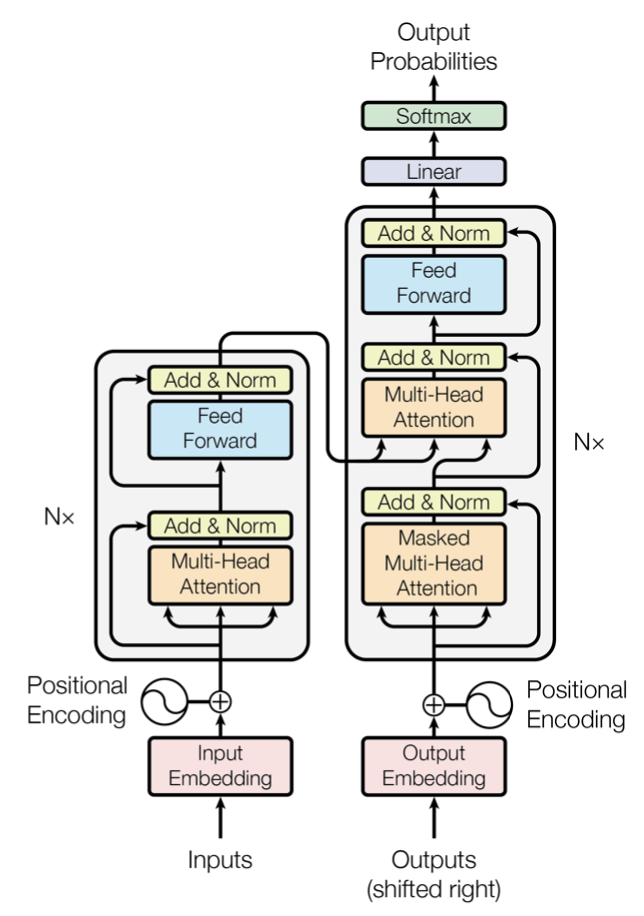
\includegraphics[width=0.5\textwidth]{figs/transform_model.png}
                \caption{Transformer model architecture - Taken from “Attention Is All You Need“}
            \end{figure}

            At a high level, the goal of the Transformer is to take an input text and predict the next word in the sequence. The input text is broken into tokens, which are typically words or parts of words. Each token is then represented as a high-dimensional vector, known as its embedding. Initially, these embeddings encode only the individual meaning of the tokens without any contextual information.

            \subsubsection{Encoder}
            The encoder consists of a stack of \(N\) identical layers, each containing two sub-layers: a multi-head self-attention mechanism and a feed-forward neural network. Furtherly, a residual connection is employed around each of the two sub-layers, followed by layer normalization. So the output of each sub-layer is \(\text{LayerNorm}(x + \text{SubLayer} (x))\), where \(\text{SubLayer}(x)\) represents the function implemented by the sub-layer.
            
            The self-attention mechanism allows the model to weigh the importance of different words in the input sequence when generating the output. The feed-forward neural network processes the output of the self-attention mechanism to produce the final hidden states of the encoder. A key feature of the encoder is that it processes all words in the input sequence in parallel, which contributes to the efficiency of the Transformer model. The output of the encoder is a sequence of vectors, each representing an input word in a high-dimensional space.

            \subsubsection{Decoder}
                The decoder, on the other hand, also consists of a stack of \(N\) identical layers, but with an additional third sublayer in each decoder layer, which performs multi-head attention over the encoder's output. This allows the decoder to focus on different parts of the encoder's output for each word in the output sequence. In the first sublayer of the decoder, self-attention is used, but with a constraint (masking) to prevent positions from attending to subsequent positions. This ensures that the predictions for position \(i\) can depend only on the known outputs at positions less than \(i\). The purpose of the decoder is to generate an output sequence one word at a time, using the encoder's output and what it has produced so far as inputs.

            \subsubsection{Attention}
                The attention mechanism is a cornerstone of the Transformer model. Its primary function is to dynamically adjust the importance of each word in the input sequence based on its context, thereby refining the embeddings of these words to capture richer meanings.

                The attention mechanism allows each token to attend to every other token in the sequence, effectively allowing the model to focus on the most relevant parts of the input when making predictions. This process is mathematically described as follows:

                \begin{equation}
                    \text{Attention}(Q, K, V) = \text{softmax}\left(\frac{QK^T}{\sqrt{d_k}}\right)V
                    \label{eq:attention}
                \end{equation}

                Here, \(Q\), \(K\), and \(V\) are the query, key, and value matrices, respectively. These matrices are derived from the input embeddings by multiplying them with learned weight matrices. The dimension \(d_k\) is the size of the key vectors and serves to scale the dot products to prevent them from growing too large.

                To understand how this works, consider a simple example: The phrases
                \begin{itemize}
                    \item "After dinner, they enjoyed a sticky \emph{date} pudding."
                    \item "She circled the \emph{date} of the concert on her calender."
                    \item "They went on their first \emph{date} to the zoo."
                \end{itemize}
                The word "date" has different meanings in each phrase, but its initial embedding would be the same. The attention mechanism helps to refine the meaning of "date" based on its context by allowing the embeddings of surrounding words to influence it.

                \textbf{Steps of the Attention Mechanism}:
                \begin{enumerate}
                    \item \textbf{Compute Query, Key, and Value Vectors:} For each embedded token \(\overrightarrow{E_i}\), we compute query (\(\overrightarrow{Q_i}\)), key (\(\overrightarrow{K_i}\)), and value (\(\overrightarrow{V_i}\)) vectors by multiplying the token's embedding with learned matrices \(W^Q\), \(W^K\), and \(W^V\):
                    \[
                    \overrightarrow{Q_i} = W^Q\overrightarrow{E_i}, \quad \overrightarrow{K_i} = W^K\overrightarrow{E_i}, \quad \overrightarrow{V_i} = W^V\overrightarrow{E_i}
                    \]

                    \item \textbf{Compute Attention Scores:} Calculate the dot products of the query vectors with all key vectors to measure how much focus each word should have on every other word, and divide by the square root of the key dimension for numerical stability:
                    \[
                    \text{Scores} = \frac{QK^T}{\sqrt{d_k}}
                    \]

                    \item \textbf{Apply Softmax Activation:} Normalize these scores using the softmax function to obtain attention weights:
                    \[
                    \text{Attention Weights} = \text{softmax}\left(\frac{QK^T}{\sqrt{d_k}}\right)
                    \]

                    \item \textbf{Compute Weighted Sum of Values:} Multiply the attention weights by the value vectors to get the final output for each token:
                    \[
                    \text{Output} = \text{softmax}\left(\frac{QK^T}{\sqrt{d_k}}\right) V
                    \]
                \end{enumerate}
                which finally leaves us with Eq. \ref{eq:attention}.
                \begin{figure}[H]
                    \centering
                    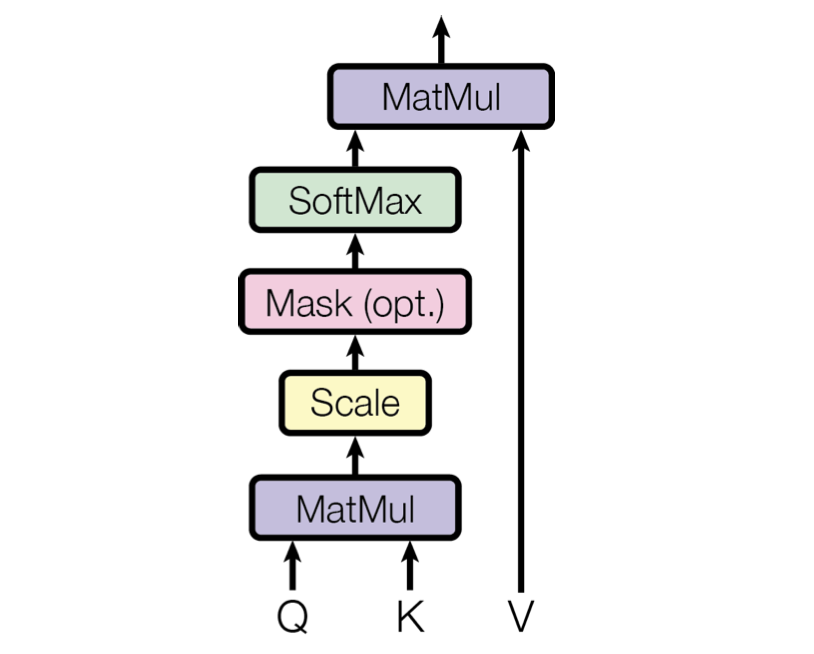
\includegraphics[width=0.6\textwidth]{figs/Scaled_dot_product.png}
                    \caption{Illustration of the Attention Mechanism - Taken from "Attention Is All You Need"}
                    \label{fig:attention_mechanism}
                \end{figure}

                This mechanism allows the model to dynamically adjust which parts of the input sequence to focus on, thereby capturing the contextual meaning of each word. This whole process is described as a single 'head' of attention, and multiple heads can be used in parallel to capture different aspects of the input sequence.

            \subsubsection{Multi-head Attention}
                Multi-head attention extends the single-head attention mechanism by allowing the model to attend to different parts of the input sequence simultaneously, capturing a variety of relationships and patterns. Instead of performing a single attention function, multi-head attention projects the queries, keys, and values into multiple subspaces and performs the attention function in each subspace independently.

                This process is mathematically described as follows:

                \begin{align}
                    \text{MultiHead}(Q, K, V) &= \text{Concat}(\text{head}_1, \ldots, \text{head}_h)W^O \\
                    \textbf{where } \text{head}_i &= \text{Attention}(QW_i^Q, KW_i^K, VW_i^V)
                \end{align}

                Here the projections are the learned parameter matrices  \(W_i^Q\), \(W_i^K\), and \(W_i^V\) for the \(i\)-th head, and \(W^O\) is the output matrix.

                \textbf{Steps of Multi-head Attention}:
                \begin{enumerate}
                    \item \textbf{Linear Projections}: Project the input embeddings into \(h\) different subspaces using learned weight matrices to create multiple sets of queries, keys, and values:
                    \[
                    Q_i = QW_i^Q, \quad K_i = KW_i^K, \quad V_i = VW_i^V
                    \]

                    \item \textbf{Parallel Attention Heads}: Apply the attention mechanism to each set of projections in parallel, producing multiple attention outputs:
                    \[
                    \text{head}_i = \text{Attention}(Q_i, K_i, V_i)
                    \]

                    \item \textbf{Concatenate and Project}: Concatenate the outputs of all attention heads and project them back to the original embedding space using a final learned matrix \(W^O\):
                    \[
                    \text{MultiHead}(Q, K, V) = \text{Concat}(\text{head}_1, \ldots, \text{head}_h)W^O
                    \]
                \end{enumerate}
                Multi-head attention allows the model to capture different aspects of the input sequence in parallel, which enhances its ability to understand complex patterns and dependencies in the data.
                \begin{figure}[H]
                    \centering
                    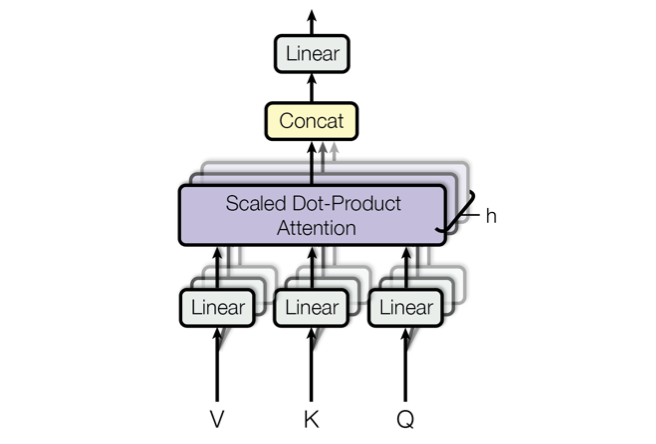
\includegraphics[width=0.6\textwidth]{figs/Multi_head_attention.png}
                    \caption{Illustration of Multi-head Attention - Taken from "Attention Is All You Need"}
                    \label{fig:multi_head_attention}
                \end{figure}
                In summary, the attention and multi-head attention mechanisms enable the Transformer model to focus on relevant parts of the input sequence dynamically, improving its ability to capture context and generate accurate predictions. These mechanisms are crucial to the model's success in various natural language processing tasks.
                                        
                
                \subsubsection{Why Transformers?}
                The Transformer model has several advantages over traditional RNNs and LSTMs, including the ability to capture long-range dependencies, parallelize computation, and scale to larger datasets. The self-attention mechanism allows the model to focus on relevant parts of the input sequence, enabling it to learn complex patterns in the data. The multi-head attention mechanism further enhances the model's ability to capture different aspects of the input sequence in parallel, improving its performance on a wide range of NLP tasks such as translation, summarization, and image captioning. This is why Transformers have become the architecture of choice for many state-of-the-art NLP models, including GPT and BERT.

            \subsection{Training and Fine-Tuning}
            The foundation of an LLM's understanding and generation of human language lies in its pre-training phase. During this stage, the model is exposed to a large corpus of text data, often encompassing a wide range of topics, genres, and styles. The primary objective of pre-training is to enable the model to learn a generalized representation of language.
            
            The pre-training is typically conducted using unsupervised learning techniques, where the model is trained on tasks like Masked Language Modeling (MLM) or Next Sentence Prediction (NSP). In MLM, for example, a percentage of the input tokens are randomly masked, and the model's objective is to predict the original tokens at these masked positions. The MLM objective can be formally represented as:
            
            \begin{equation}
            \mathcal{L}_{\text{MLM}} = -\sum_{i \in \mathcal{M}} \log p(x_i | x_{\backslash \mathcal{M}})
            \end{equation}
            
            where $\mathcal{M}$ is the set of masked positions, $x_i$ is the original token at position $i$, and $x_{\backslash \mathcal{M}}$ represents the input with masked tokens.
            \vspace*{0.2cm}

            Following pre-training, LLMs undergo a fine-tuning phase, wherein the model is specialized to perform specific NLP tasks. This phase involves training the pre-trained model on a smaller, task-specific dataset, allowing the model to adjust its weights to better perform the target task.
            
            The fine-tuning process can be represented as a continuation of the training process, optimizing the following objective:
            
            \begin{equation}
            \mathcal{L}_{\text{fine-tune}} = -\sum_{(x,y) \in \mathcal{D}_{\text{task}}} \log p(y | x; \theta_{\text{pre-train}} + \Delta\theta)
            \end{equation}
            
            where $\mathcal{D}_{\text{task}}$ is the task-specific dataset, $(x,y)$ are the input-output pairs, $\theta_{\text{pre-train}}$ are the parameters learned during pre-training, and $\Delta\theta$ represents the parameter updates during fine-tuning.
            \vspace*{0.2cm}

            Fine-tuning LLMs presents challenges such as catastrophic forgetting and overfitting, particularly when the task-specific dataset is small. Various strategies, including careful learning rate selection, regularization techniques, and the use of adapters, are employed to mitigate these issues.
\chapter{Literature Review}

\section{Overview of Large Language Models}

\section{Linear Algebra in Machine Learning}

\section{Previous Studies on LLM Compression and Optimization}
\chapter{Methodology}

\section{RAG Chatbot: Study Buddy}

    \subsection{Motivation}
    As a teaching assistant, I have observed that students frequently resort to using chatbots like ChatGPT for quick answers to their questions. However, these chatbots often provide generic responses that may not be sufficiently helpful for academic purposes, as they lack the specificity and depth required for effective studying. This observation underscores a gap in the effectiveness of current chatbot solutions in educational contexts.

    The Retrieval-Augmented Generation (RAG) model addresses this gap by combining a retriever and a generator, thereby enabling the delivery of more detailed and context-specific information. 
    
    To gain practical experience with large language models (LLMs) and their application in real-world language processing tasks, I developed a chatbot inspired by a project at BSS - Aarhus University (Appendix \ref{appendix:Bergenholtz}). This chatbot, utilizing the RAG model \cite{lewis2020RAG}, serves as a 'Study Buddy' to assist students in understanding complex topics, providing quick and relevant answers, and enhancing their learning experience for challenging subjects.

    \subsection{Development and Environment Tools}
    The implementation of the RAG chatbot was accomplished using the following tools and technologies:
    \begin{itemize}
        \item \textbf{OpenAI API:} Utilized to access the GPT-4 model for the chatbot's generation capabilities.
        \item \textbf{Astra DB:} Employed for storing and managing the data used by the retriever component.
        \item \textbf{DataStax RAGstack:} A curated stack of leading open-source software designed to facilitate the implementation of the RAG pattern in production-ready applications using Astra Vector DB as a vector store.
        \item \textbf{Langchain:} An open-source framework used for developing applications powered by LLMs.
        \item \textbf{Streamlit:} An open-source Python framework used for building and deploying data applications with minimal code.
    \end{itemize}

    \subsection{Implementation Steps}
    The development of the RAG chatbot involves the following steps:
    \begin{enumerate}
        \item \textbf{Chatbot Interface:} Designing and creating a user-friendly interface for users to interact with the chatbot.
        \item \textbf{Generator Component:} Implementing the generator component to provide responses based on the GPT-4 model.
        \item \textbf{Retriever Component:} Developing the retriever component to search for relevant information based on user queries.
        \item \textbf{Integration:} Integrating the retriever and generator components to create a functional RAG chatbot.
        \item \textbf{PDF Uploader:} Implementing a feature that allows users to upload their own materials, enabling more meaningful and contextual responses.
        \item \textbf{Deployment:} Deploying the chatbot on a cloud platform to make it publicly accessible.
    \end{enumerate}
        
    The theoretical workflow of the RAG chatbot is illustrated in Figure \ref{fig:rag_chatbot}. The process begins with the user inputting a query, which is then processed by the retriever to find relevant information. This information provides context based on the user's query. Subsequently, the generator creates a response using an embedded prompt template, the retrieved information, and the user's query, thereby providing the user with a detailed and specific answer.
    
    \begin{figure}[H]
        \centering
        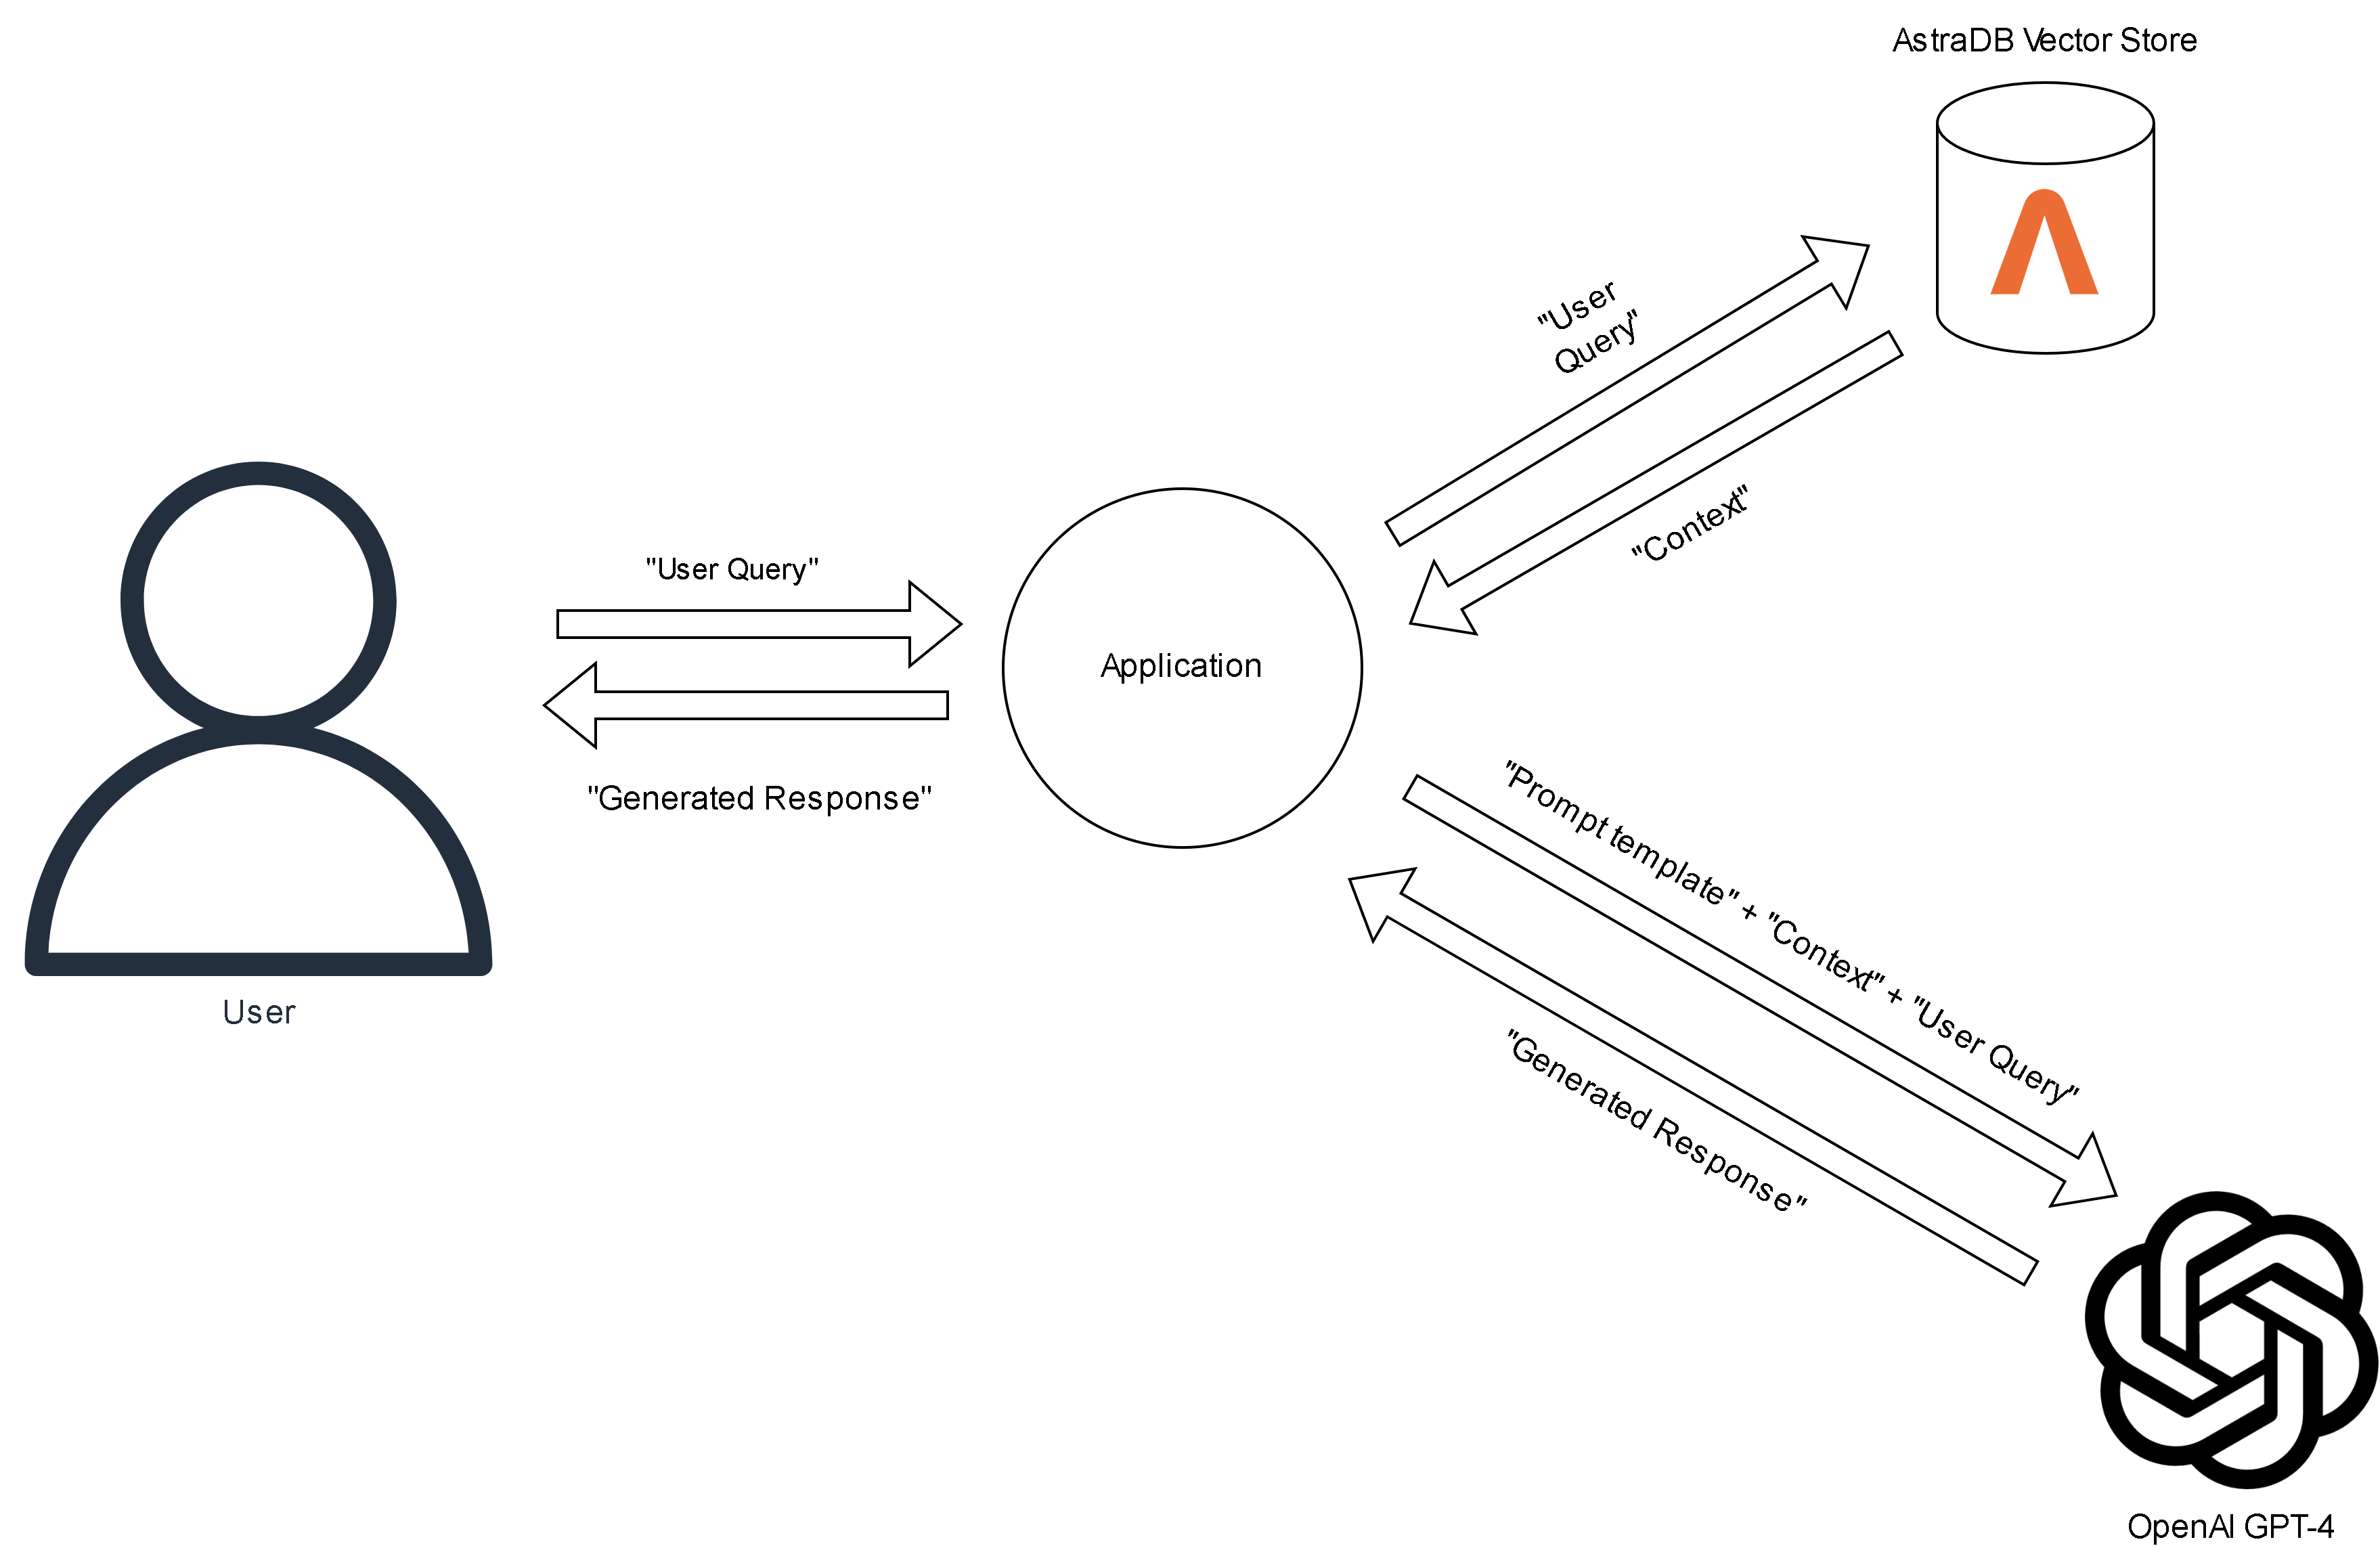
\includegraphics[width=0.8\textwidth]{figs/Chatbot_process.png}
        \caption{Diagram of Query Process}
        \label{fig:rag_chatbot}
    \end{figure}


    



\section{LLM Optimization}
    Optimizing Large Language Models (LLMs) for efficiency and performance without compromising their effectiveness is a critical area of research in the field of artificial intelligence. Various techniques have been developed to address this challenge, each employing unique strategies to reduce computational resources, decrease model size, and maintain, if not improve, the model's performance. This section explores the general methodologies applied in the optimization of LLMs, focusing particularly on model compression techniques. Among these, Low-Rank Approximation stands out as a highly effective approach. This technique leverages the mathematical properties of matrices to approximate the original model parameters with fewer components, thereby possibly reducing the model's computations and resource requirements.

    \subsection{Optimization Techniques for Large Language Models}
        Optimization strategies for Large Language Models (LLMs) are crucial for improving computational efficiency and model efficacy. These strategies are generally divided into two primary types: model pruning and parameter sharing.

        \subsubsection{Model Pruning}
        Model pruning aims to reduce the model's complexity and size effectively without substantial loss in performance. It involves systematically eliminating parameters or connections within the model that are least consequential to the output, thereby enhancing operational efficiency and making the model more adaptable for use in environments with limited resources.

        \subsubsection{Parameter Sharing}
        Conversely, parameter sharing utilizes the model's existing parameters across various parts of the model or different tasks. This method optimizes the use of the model's capacity, enabling multifunctional performance without an increase in parameter count.

        \subsubsection{Focus on Low-Rank Approximation}
        This thesis will specifically focus on model pruning techniques, with a particular emphasis on low-rank approximation. This approach approximates large matrices or tensors with ones of a lower rank, reducing the number of components and computational demands while preserving the model's critical information processing capabilities.


\section{Case Study: Low-Rank Approximation}
    To assess the effectiveness of low-rank approximation in compressing LLMs, we consider Facebook's the BART-Base model (\cite{lewis2019bart}) as a case study. BART is a transformer-based LLM that has been widely used for various natural language processing tasks such as summarization.%\ref{sec:bart}

    This thesis focuses on applying low-rank approximation specifically to the attention matrices. This choice stems from their pivotal role in the transformer architecture. These matrices, which help the model assess the relevance of different words within the input data, tend to be large and often encapsulate redundant information (\cite{aghajanyan2020intrinsic}). %By reducing the dimensionality of these matrices, we preserve the model's ability to perform complex relational reasoning with less computational overhead, thus maintaining efficacy in summarization tasks while enhancing efficiency.

    By applying low-rank approximation to the attention weight matrices of the BART-base model, we aim to explore the possibility in reducing computational complexity and storage requirements while preserving its performance on a summarization task.
    \subsection{Implementation Steps}
        The implementation of low-rank approximation for BART involves the following steps:
        
        \begin{enumerate}
            \item \textbf{Singular Value Decomposition (SVD):} The attention weight matrices (Key, Query, Value, and Output) of the model are decomposed using SVD to obtain the low-rank approximation.
            \[
            \begin{array}{c}
                Q \\[0.2cm] % adds 0.5 cm space after this row
                V \\[0.2cm] % adds 0.5 cm space after this row
                K \\[0.2cm]
                O
            \end{array}
            \xrightarrow[\text{SVD}]{\hspace*{1cm}}
            \begin{array}{c}
                U_q \ \Sigma_q \ V_q^T \\[0.2cm] % adds 0.5 cm space after this row
                U_v \ \Sigma_v \ V_v^T \\[0.2cm] % adds 0.5 cm space after this row
                U_k \ \Sigma_k \ V_k^T \\[0.2cm]
                U_o \ \Sigma_o \ V_o^T

            \end{array}
            \]

            \item \textbf{Custom Layer Implementation:} A custom layer is implemented to replace the original attention layers with the low-rank approximation.
            \begin{figure}[H]
                \centering
                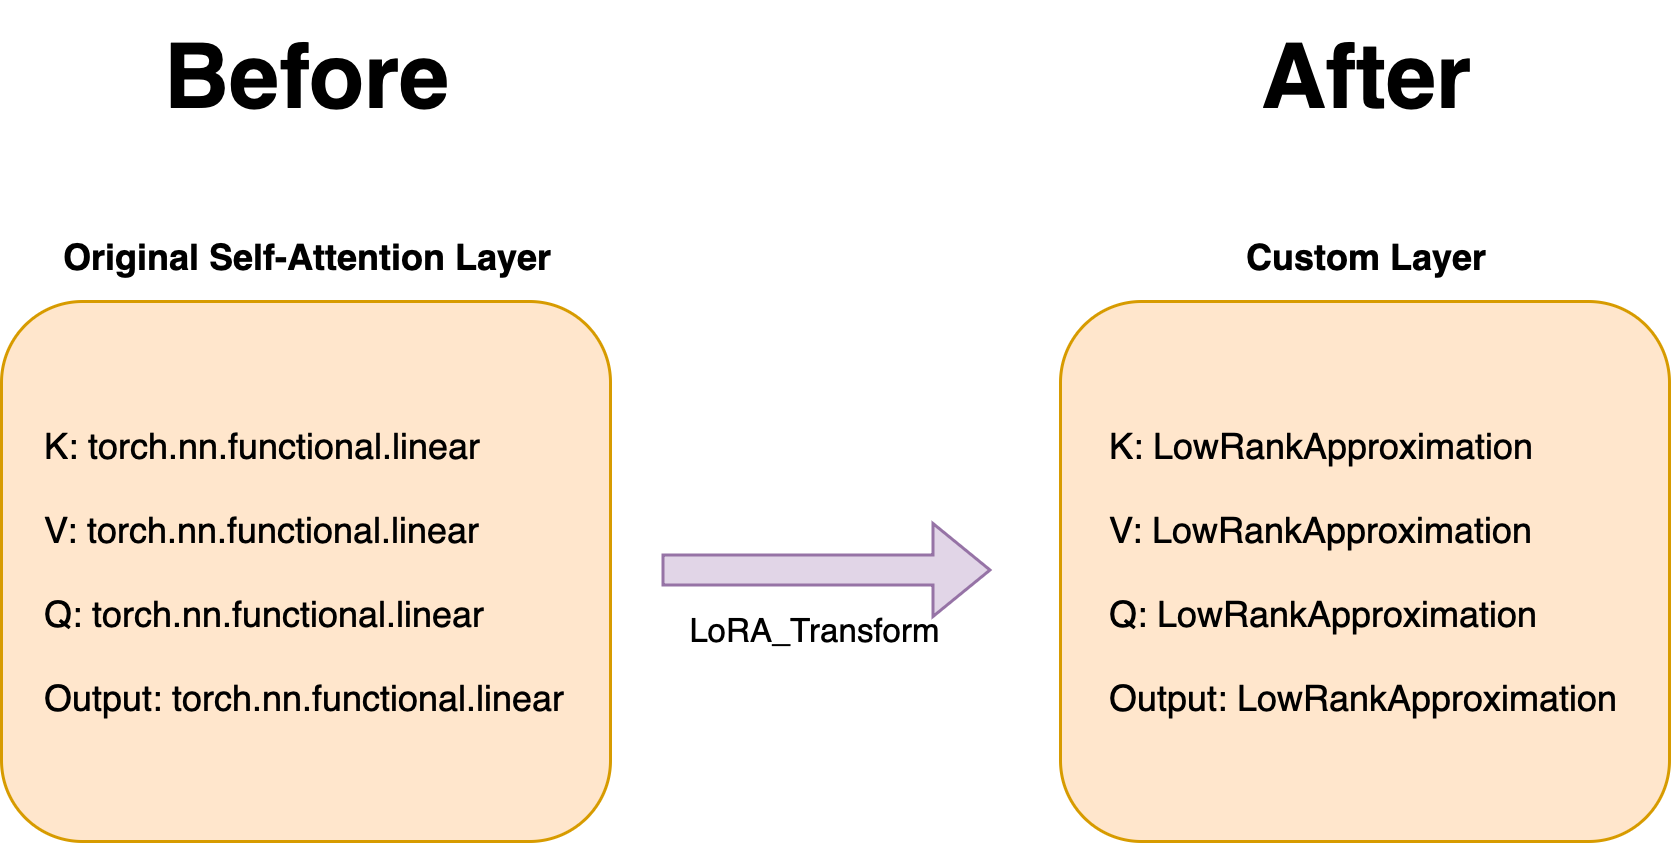
\includegraphics[width=0.7\textwidth]{figs/before-after.png}
                \caption{Components in attention layers replaced with their custom low-rank approximation}
                \label{fig:lora_implementation}
            \end{figure}
        \end{enumerate}
        
        
        
    \subsection{Evaluation Metrics}\label{sec:evaluation_metrics}
        The approximated model is evaluated based on:
        \begin{enumerate}
        \item ROUGE scores (\cite{lin-2004-rouge}): How well does the approximated model perform in comparison to the original BART-Base model on the summarization task? From which rank does the model start to lose performance?
        \item Computational efficiency: How does the approximated model compare to the original BART-Base model in terms of computational resources required?
        \item Cosine similarity: How well does the approximated model maintain the semantic properties of the original model?
        \item Comparing some of the summaries generated by the compressed model with the original BART-Base model and the reference summaries using the Samsum dataset (\cite{gliwa-etal-2019-samsum}).
        \begin{figure}[H]
            \centering
            \includegraphics[width=0.6\textwidth]{figs/dialogue.png}
            \caption{SamSum Dataset \texttt{test[0]} dialogue and reference summary}
            \label{fig:SamSum_Example}
        \end{figure}
        \end{enumerate}

        \subsection{Appropriate Rank Selection}
            In Section \ref{sec:reduction_storage}, we established the criterion for selecting an appropriate rank \(k\) to achieve computational efficiency and storage reduction. The criterion is given by:
            
            \[
            k < \frac{\sqrt{4mn + (m+n)^2} - m - n}{2}
            \]
            
            where \(m\) and \(n\) are the dimensions of the original matrix we wish to approximate with a low-rank representation.
            
            \textbf{BART-base Model:}\\
            For the BART-base model, the attention matrices have dimensions \(m = n = 768\). We know this by inspecting the model's architecture (Appendix \ref{appendix:BART}).\\
            Therefore, the rank \(k\) for the approximation should satisfy:
            \[
            k < \frac{\sqrt{4 \times 768 \times 768 + (768 + 768)^2} - 768 - 768}{2} \approx 318
            \]
            
            \label{appropriate_rank}to achieve a reduction in computational complexity and storage requirements.

            \textbf{BART-large Model:}\\
            Similarly, for the BART-large model, the attention matrices have dimensions \(m = n = 1024\). Therefore, the rank \(k\) for the approximation should satisfy:
            \[
            k < \frac{\sqrt{4 \times 1024 \times 1024 + (1024 + 1024)^2} - 1024 - 1024}{2} \approx 424
            \]
            To determine the feasibility of low-rank approximation for the two BART models, we will evaluate the approximated model at various ranks and observe the impact on the ROUGE scores and the other metrics mentioned in section \ref{sec:evaluation_metrics}. This evaluation will help us understand the trade-offs between rank reduction and model performance.
            

            

        %\textbf{Rank Selection:} The rank of the approximation is chosen based on the observed spectrum decay of the ROUGE-scores, ensuring a balance between speed and task performance retention.


\chapter{Implementation}\label{chap:implementation}
This chapter details the implementation of the Retrieval-Augmented Generation (RAG) Chatbot and the low-rank approximation technique applied to the BART model. The implementation process encompasses the development of the chatbot interface, the integration of generator and retriever components, the setup for handling user-uploaded documents, and the deployment of the chatbot. Additionally, the chapter covers the importation and preprocessing of the SamSum dataset, fine-tuning the BART model, implementing custom low-rank layers, and traversing the model to apply low-rank approximations. Each step is meticulously documented with code snippets and explanations to provide a comprehensive understanding of the implementation.
\section{RAG Chatbot}
The development of the RAG Chatbot, named "Study Buddy," aims to address the limitations of current chatbot solutions in educational contexts. Leveraging the Retrieval-Augmented Generation (RAG) model, this chatbot integrates advanced retrieval mechanisms with generative capabilities to provide students with context-specific and detailed responses. This section details the implementation process, including the creation of the user interface, the integration of the generator and retriever components, the setup for handling user-uploaded documents, and the deployment strategy. Through these steps, the Study Buddy chatbot is designed to enhance students' learning experiences by delivering accurate and relevant information efficiently.
    \subsection{Chatbot Interface}
        The chatbot interface was developed using the \texttt{Streamlit} library, which provides a simple and interactive way to create web applications. The interface allows users to interact with the RAG chatbot by entering a question in the input field and receiving the corresponding answer from the model. The chatbot interface was designed to be user-friendly and intuitive, enabling users to easily communicate with the chatbot and obtain relevant information.
        \begin{figure}[H]
            \centering
            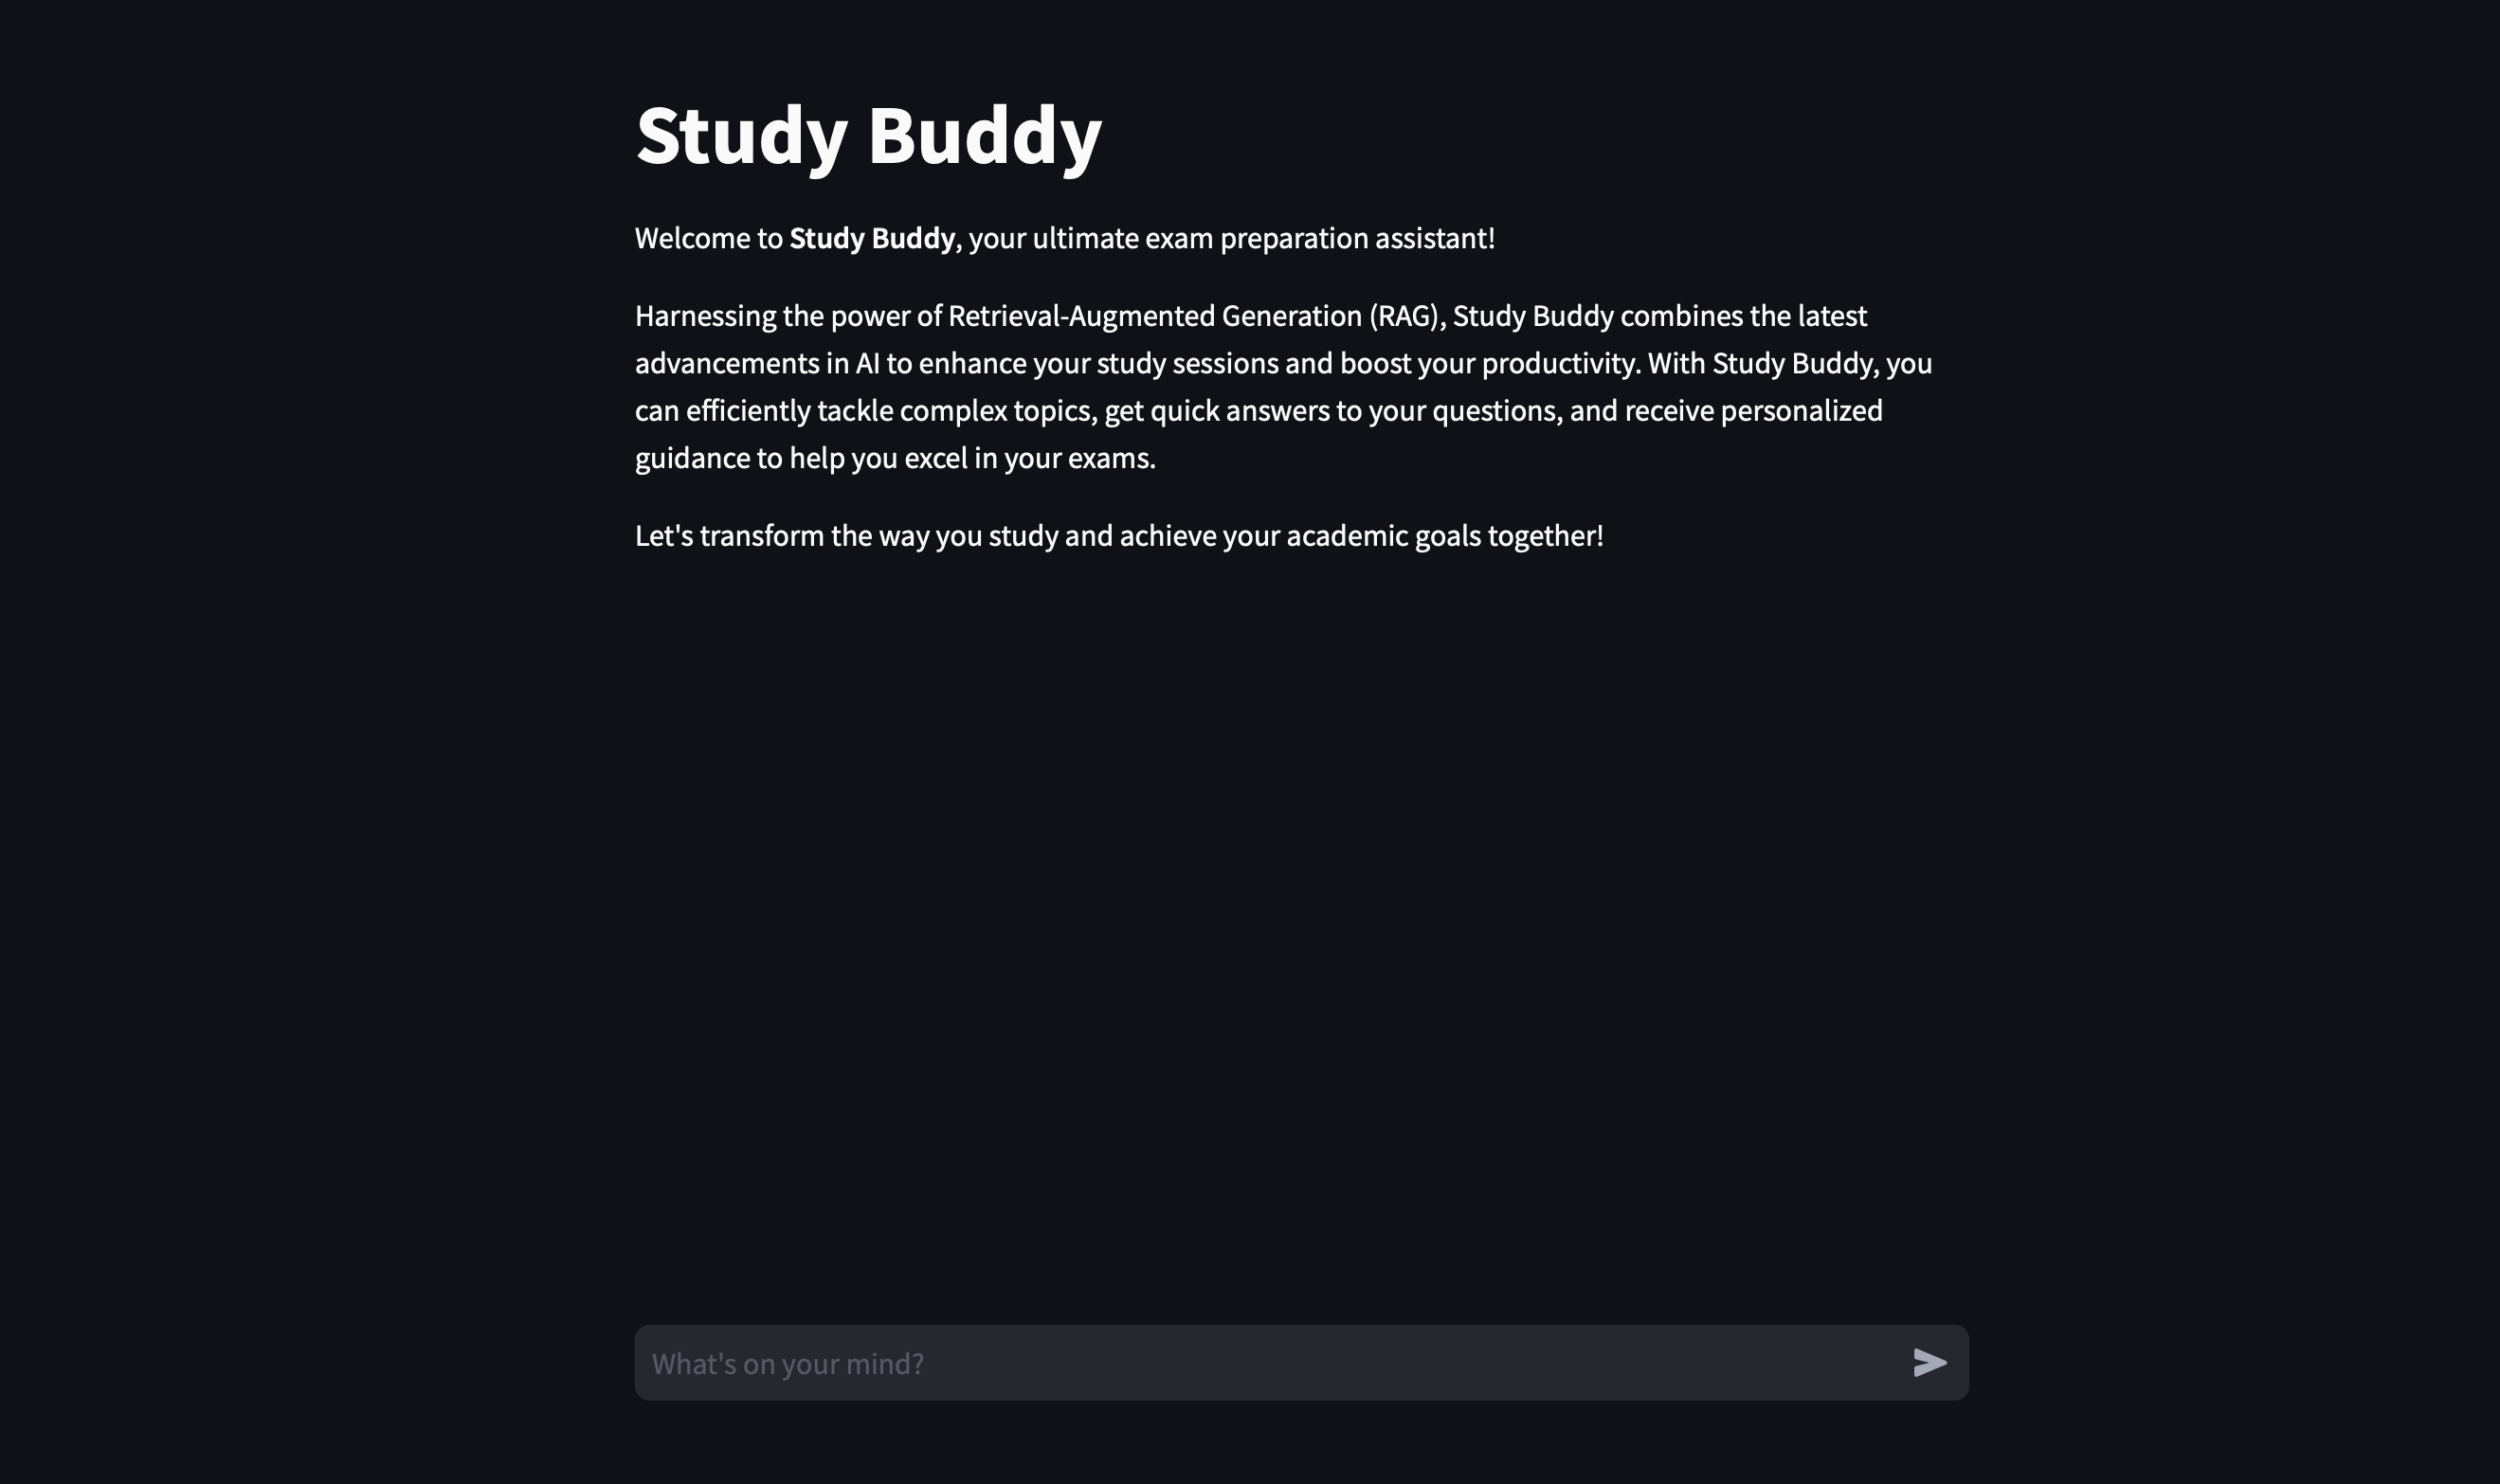
\includegraphics[width=0.8\textwidth]{figs/interface.png}
            \caption{RAG Chatbot Interface}
            \label{fig:chatbot_interface}
        \end{figure}
            
            The chatbot interface displays a title, description and input field for user queries using the \texttt{st.title}, \texttt{st.markdown} and \texttt{st.chat\_input} functions respectively. The title introduces the chatbot as "Study Buddy," while the description provides an overview of the chatbot's capabilities and features. By using the \texttt{Streamlit} library, the chatbot interface can be created by just a few lines of code.

\subsection{Generator Component}
The generator component of Study Buddy was implemented using the \texttt{Langchain} library, which provides ready-to-use methods to call OpenAI's GPT-4 model. Streamlit reruns the code in the \texttt{app.py} file every time a user interacts with the chatbot. The following code snippets demonstrate how the generator calls the GPT-4 model and generates responses to user queries.

\begin{listing}[H]
\begin{minted}[fontsize=\footnotesize]{python}
from langchain_openai import ChatOpenAI

# Cache OpenAI Chat Model for reuse
@st.cache_resource()
def get_chat_model():
    return ChatOpenAI(
        temperature=0.3,
        model='gpt-4',
        streaming=True,
        verbose=True
    )
chat_model_instance = get_chat_model()
\end{minted}
\caption{Caching the OpenAI Chat Model}
\label{listing:Cache_Chat_Model}
\end{listing}

The code snippet in listing \ref{listing:Cache_Chat_Model} details the implementation of the generator component for the Study Buddy chatbot, leveraging the \texttt{Langchain} library to interface with OpenAI's GPT-4 model. The generator component is responsible for producing the responses to user queries.

\textbf{Key Elements of the Code:}
\begin{itemize}
    \item \texttt{ChatOpenAI}: This class from the \texttt{langchain\_openai} module facilitates interaction with OpenAI's GPT-4 model.
    \item \texttt{@st.cache\_resource}: This Streamlit decorator caches the chat model instance, ensuring efficient reuse across multiple interactions without the need to reinitialize it each time.
    \item \texttt{temperature}: A parameter that controls the randomness of the model's responses, with a value of 0.3 indicating a balance between creativity and determinism.
    \item \texttt{model='gpt-4'}: Specifies the use of the GPT-4 model for generating responses.
    \item \texttt{streaming=True}: Enables streaming of the model's output, allowing for real-time response generation.
    \item \texttt{verbose=True}: Provides detailed logs of the model's operations for debugging and transparency.
\end{itemize}

\textbf{Explanation of Functionality:}
\begin{enumerate}
    \item \textbf{Caching the Chat Model:} The \texttt{get\_chat\_model()} function initializes and caches an instance of the GPT-4 model with specific parameters. By caching this instance, the system ensures that the model does not need to be reloaded each time a user interacts with the chatbot, thereby improving efficiency and response times.
    \item \textbf{Model Parameters:} The temperature parameter is set to 0.3, which strikes a balance between generating creative responses and maintaining consistency. The \texttt{streaming=True} parameter enables the model to stream responses in real-time, providing a more interactive and immediate user experience. The \texttt{verbose=True} parameter allows for detailed logging, which is useful for monitoring the chatbot's operations and debugging issues.
\end{enumerate}

This setup ensures that the generator component efficiently interacts with the GPT-4 model to generate responses to user queries. The caching mechanism optimizes performance by reusing the model instance across multiple interactions.

        
\subsection{Retriever Component}
The retriever component of Study Buddy was implemented using the \texttt{Langchain} library to retrieve the \(k = 5\) most relevant documents from the Astra DB Vector Store.

\begin{listing}[H]
\begin{minted}[fontsize=\footnotesize]{python}
from langchain_community.vectorstores import AstraDB
from langchain_openai import OpenAIEmbeddings

# Cache the Astra DB Vector Store for reuse
@st.cache_resource(show_spinner='Connecting to AstraDB')
def get_vector_store():
    vector_store_instance = AstraDB(
        embedding=OpenAIEmbeddings(),
        collection_name="datastax",
        api_endpoint=st.secrets['ASTRA_API_ENDPOINT'],
        token=st.secrets['ASTRA_TOKEN']
    )
    return vector_store_instance
vector_store_instance = get_vector_store()

# Cache the Retriever for reuse
@st.cache_resource(show_spinner='Initializing retriever')
def get_retriever():
    retriever_instance = vector_store_instance.as_retriever(
        search_kwargs={"k": 5}
    )
    return retriever_instance
retriever_instance = get_retriever()
\end{minted}
\caption{Caching the Astra DB Vector Store and Retriever}
\label{listing:Cache_Retriever}
\end{listing}

The code snippet in listing \ref{listing:Cache_Retriever} demonstrates the implementation of the retriever component for the Study Buddy chatbot. The \texttt{Langchain} library is utilized to connect to the Astra DB Vector Store, which is a database optimized for vector searches. The retriever component is responsible for identifying and retrieving the most relevant documents based on the user's query.

\textbf{Key Elements of the Code:}
\begin{itemize}
    \item \texttt{AstraDB}: This class from the \texttt{langchain\_community.vectorstores} module is used to create an instance of the vector store.\footnote{The vector store was configured in the DataStax Astra DB cloud service to use cosine similarity for semantic searches.}
    It requires an embedding model, collection name, API endpoint, and a token for authentication.
    \item \texttt{OpenAIEmbeddings}: This class from the \texttt{langchain\_openai} module provides the embedding model used to convert text into numerical vectors that the vector store can handle.
    \item \texttt{@st.cache\_resource}: This Streamlit decorator caches the resources, ensuring that the vector store and retriever instances are reused efficiently across different runs of the application. This caching mechanism helps to optimize performance by avoiding redundant connections and initializations.
    \item \texttt{get\_vector\_store()}: This function initializes and returns an instance of the vector store by connecting to Astra DB using the provided API endpoint and token.
    \item \texttt{get\_retriever()}: This function initializes and returns an instance of the retriever, configured to fetch the top \(k = 5\) most relevant documents based on the user's query.
\end{itemize}

\textbf{Explanation of Functionality:}
\begin{enumerate}
    \item \textbf{Connecting to Astra DB:} The \texttt{get\_vector\_store()} function creates a connection to the Astra DB Vector Store using the OpenAI embeddings for document vectorization. The connection details, such as the API endpoint and token, are securely retrieved from the Streamlit secrets configuration.
    \item \textbf{Initializing the Retriever:} The \texttt{get\_retriever()} function sets up the retriever to query the vector store. The retriever is configured to return the top 5 relevant documents, which helps in providing contextually accurate responses to user queries.
\end{enumerate}

This setup ensures that the retriever component can efficiently access and retrieve relevant information, enhancing the chatbot's ability to deliver detailed and context-specific answers.

\subsection{Integration of Generator and Retriever}
The generator and retriever components were integrated to provide a comprehensive response to user queries. The following code snippet demonstrates how the generator and retriever components work together to generate responses based on the user's input.

\begin{listing}[H]
\begin{minted}[fontsize=\footnotesize]{python}
from langchain.schema.runnable import RunnableMap

input_data = RunnableMap({
        'context': lambda x: retriever_instance.get_relevant_documents(x['question']),
        'question': lambda x: x['question']
    })
response_chain = input_data | chat_prompt | chat_model_instance
\end{minted}
\caption{Integration of Generator and Retriever}
\label{listing:Integration_Generator_Retriever}
\end{listing}

The code snippet in listing \ref{listing:Integration_Generator_Retriever} illustrates the integration of the generator and retriever components for the Study Buddy chatbot. This integration ensures that user queries are processed using both components to provide contextually accurate and comprehensive responses.

\textbf{Key Elements of the Code:}
\begin{itemize}
    \item \texttt{RunnableMap}: This class is used to map the inputs (context and question) to the necessary functions for processing.
    \item \texttt{retriever\_instance.get\_relevant\_documents}: This function retrieves the most relevant documents from the vector store based on the user's query.
    \item \texttt{chat\_prompt}: A predefined template that formats the retrieved context and user question for the generator.
    \item \texttt{chat\_model\_instance}: The cached instance of the GPT-4 model used for generating responses.
\end{itemize}

\textbf{Explanation of Functionality:}
\begin{enumerate}
    \item \textbf{Input Data Mapping:} The \texttt{RunnableMap} is used to create a mapping of inputs, where the 'context' key is assigned a lambda function that retrieves relevant documents based on the user's question, and the 'question' key simply maps the user's question.
    \item \textbf{Response Chain Creation:} The \texttt{response\_chain} is constructed by chaining the input data through the chat prompt and the chat model instance. This chain ensures that the user's question is enriched with relevant context before generating the final response.
    \item \textbf{Generating Responses:} When invoked, the \texttt{response\_chain} processes the inputs by first retrieving the relevant documents, then formatting them using the chat prompt, and finally generating a comprehensive response using the GPT-4 model.
\end{enumerate}

This integration of the generator and retriever components ensures that the Study Buddy chatbot can deliver detailed and contextually relevant answers to user queries, enhancing its utility as an exam preparation assistant.

\subsection{PDF Uploader}
The PDF uploader component allows users to upload course materials, lecture notes, or other relevant documents to the Study Buddy chatbot. The uploaded documents are stored in the Astra DB Vector Store, enabling the chatbot to retrieve and reference them when responding to user queries.

\begin{listing}[H]
\begin{minted}[fontsize=\footnotesize]{python}
# Sidebar for document upload
with st.sidebar:
    with st.form('upload_form'):
        uploaded_file = st.file_uploader('Upload a document for enhanced context', type=['pdf'])
        submit_button = st.form_submit_button('Save to AstraDB')
        if submit_button:
            process_and_vectorize_document(uploaded_file, vector_store_instance)
\end{minted}
\caption{PDF Uploader Interface}
\label{listing:PDF_Uploader}
\end{listing}
The code snippet in listing \ref{listing:PDF_Uploader} creates an interface within the Streamlit sidebar for uploading PDF documents. This interface allows users to upload course materials, lecture notes, or other relevant documents, which are then processed and stored in the Astra DB Vector Store.

\begin{listing}[H]
\begin{minted}[fontsize=\footnotesize]{python}
# Function to process and vectorize uploaded documents into Astra DB
def process_and_vectorize_document(uploaded_file, vector_db):
    if uploaded_file is not None:
        
        # Create a temporary file to store the uploaded document
        temp_dir = tempfile.TemporaryDirectory()
        temp_file_path = os.path.join(temp_dir.name, uploaded_file.name)
        with open(temp_file_path, 'wb') as temp_file:
            temp_file.write(uploaded_file.getvalue())

        # Load the PDF file
        document_pages = []
        pdf_loader = PyPDFLoader(temp_file_path)
        document_pages.extend(pdf_loader.load())

        # Initialize text splitter
        splitter = RecursiveCharacterTextSplitter(
            chunk_size=1500,
            chunk_overlap=100
        )

        # Split the document and add it to the vector store
        split_pages = splitter.split_documents(document_pages)
        vector_db.add_documents(split_pages)
        st.info(f"{len(split_pages)} pages have been loaded into the database.")
\end{minted}
\caption{Processing and Vectorizing Uploaded Documents}
\label{listing:Process_Vectorize_Documents}
\end{listing}

The code snippet in \ref{listing:Process_Vectorize_Documents} defines a function that processes and vectorizes uploaded PDF documents, storing them in the Astra DB Vector Store. This function is crucial for enabling the chatbot to retrieve and reference user-uploaded materials when generating responses.

\textbf{Key Elements of the Code:}
\begin{itemize}
    \item \texttt{tempfile.TemporaryDirectory()}: Creates a temporary directory to store the uploaded file.
    \item \texttt{open(temp\_file\_path, 'wb')}: Writes the uploaded file to the temporary directory.
    \item \texttt{PyPDFLoader}: Loads the PDF document into memory.
    \item \texttt{RecursiveCharacterTextSplitter}: Splits the document into smaller chunks for vectorization.
    \item \texttt{vector\_db.add\_documents}: Adds the vectorized document chunks to the Astra DB Vector Store.
    \item \texttt{st.info}: Displays an information message indicating the number of pages processed and loaded into the database.
\end{itemize}

\textbf{Explanation of Functionality:}
\begin{enumerate}
    \item \textbf{Temporary File Storage:} The uploaded PDF document is stored temporarily to facilitate processing.
    \item \textbf{Document Loading:} The PDF document is loaded into memory using the \texttt{PyPDFLoader} class.
    \item \textbf{Text Splitting:} The loaded document is split into smaller chunks using the \texttt{RecursiveCharacterTextSplitter} class. This step is necessary to manage large documents and prepare them for vectorization.
    \item \textbf{Vectorization and Storage:} The split document chunks are vectorized and added to the Astra DB Vector Store. This enables efficient retrieval and reference by the chatbot when responding to user queries.
    \item \textbf{User Feedback:} A message is displayed to inform the user about the number of pages successfully processed and loaded into the database.
\end{enumerate}

This comprehensive approach ensures that the uploaded documents are effectively processed and made available for contextual responses, significantly enhancing the chatbot's utility and relevance.

\subsection{Deployment}
The Study Buddy chatbot was deployed using the Streamlit sharing platform, which provides a simple and efficient way to host and share Streamlit applications. The deployment process involved uploading the application code to the Streamlit sharing platform and configuring the necessary settings to make the chatbot publicly accessible.
\begin{figure}[H]
    \centering
    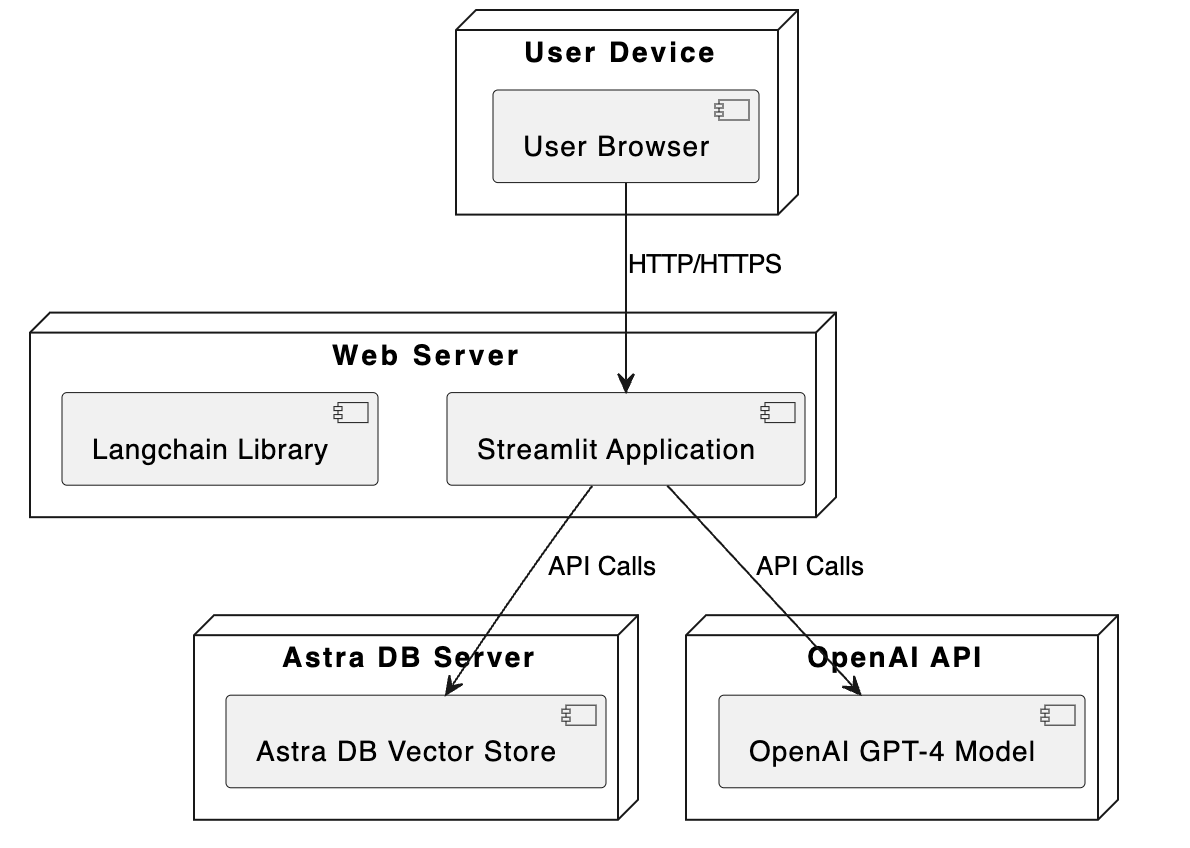
\includegraphics[width=0.8\textwidth]{figs/deployment.png}
    \caption{Deployment diagram of the Study Buddy RAG chatbot.}
    \label{fig:deployment}
\end{figure}
The deployment diagram illustrated in Figure \ref{fig:deployment} shows the architecture of the Retrieval-Augmented Generation (RAG) chatbot named \textit{Study Buddy}. This chatbot is designed to assist students in their studies by providing detailed and contextually relevant answers to their questions.

\subsubsection*{Components}

\begin{itemize}
    \item \textbf{User Device:}
    \begin{itemize}
        \item \textit{User Browser:} The interface through which users interact with the Study Buddy chatbot. Users enter their queries and receive responses via a web browser.
    \end{itemize}
    \item \textbf{Web Server:}
    \begin{itemize}
        \item \textit{Streamlit Application:} The front-end of the chatbot, developed using Streamlit. This component handles user interactions, displays the chat interface, and processes user inputs.
        \item \textit{Langchain Library:} Integrated within the Streamlit application, this library manages interactions with the OpenAI API and Astra DB. It facilitates the retrieval of relevant documents and the generation of responses.
    \end{itemize}
    \item \textbf{Astra DB Server:}
    \begin{itemize}
        \item \textit{Astra DB Vector Store:} A highly optimized vector database provided by DataStax, used to store and manage the contextual data required by the chatbot for generating precise and relevant answers.
    \end{itemize}
    \item \textbf{OpenAI API:}
    \begin{itemize}
        \item \textit{OpenAI GPT-4 Model:} The backend service provided by OpenAI, which generates human-like responses based on the input queries and contextual information retrieved from the Astra DB.
    \end{itemize}
\end{itemize}

\subsection{Connections}

\begin{itemize}
    \item \textbf{User Device to Web Server:} The user's browser communicates with the Streamlit application over HTTP/HTTPS protocols. This connection allows the user to send queries and receive responses.
    \item \textbf{Web Server to Astra DB Server:} The Streamlit application makes API calls to the Astra DB Vector Store to retrieve relevant documents based on the user's query.
    \item \textbf{Web Server to OpenAI API:} The Streamlit application also makes API calls to the OpenAI GPT-4 Model to generate detailed and contextually enriched responses.
\end{itemize}

This deployment architecture ensures that the chatbot can efficiently handle user queries by leveraging advanced natural language processing capabilities and a robust database for contextual data retrieval. The integration of these components enables \textit{Study Buddy} to provide accurate and helpful study assistance to users.

\section{Case Study: Low-Rank Approximation of BART model}
This section explores the application of low-rank approximation techniques to the BART model, focusing on both the base and large versions. By reducing the dimensionality of the attention weight matrices, the goal is to decrease computational complexity and storage requirements while maintaining performance in summarization tasks. The implementation process includes importing and preprocessing the SamSum dataset, fine-tuning the BART model, creating custom low-rank layers, and traversing the model to apply these approximations. Evaluation metrics, such as ROUGE scores and computational efficiency, are used to assess the effectiveness of this approach. This case study provides in the effectiveness of low-rank approximation of the BART model for dialogue summarization tasks.

    \subsection{Importing the Model}
        The BART-base model was imported from the Hugging Face platform using the \texttt{transformers} library.
        \begin{listing}[H]
            \begin{minted}[fontsize=\footnotesize]{python}
model_checkpoint = "facebook/bart-base"
model = AutoModelForSeq2SeqLM.from_pretrained(model_checkpoint)
            \end{minted}
            \caption{Importing the BART-base model}
            \label{listing:Importing_BART}
        \end{listing}
    
        \subsection{Dataset Preprocessing}

The SamSum dataset was imported and preprocessed to facilitate the training and evaluation of the BART-base model. The dataset comprises conversations crafted and documented by linguists proficient in English, which were subsequently annotated with summaries. The preprocessing steps included tokenization, truncation, and padding to ensure uniform input sizes for the model.

\subsubsection{Importing the Dataset}

First, the necessary libraries was imported and then the SamSum dataset was loaded using the \texttt{datasets} library:

\begin{listing}[H]
\begin{minted}[fontsize=\footnotesize]{python}
from datasets import load_dataset

raw_datasets = load_dataset("samsum")
\end{minted}
\caption{Loading the SamSum dataset}
\label{listing:Loading_SamSum}
\end{listing}

The \texttt{load\_dataset} function fetches the SamSum dataset, which contains dialogues and their corresponding summaries.

\subsubsection{Setting Maximum Lengths}

To ensure that the input and target sequences fit within the model's constraints, we set the maximum lengths for input and target sequences:

\begin{listing}[H]
\begin{minted}[fontsize=\footnotesize]{python}
max_input_length = 512
max_target_length = 128
\end{minted}
\caption{Setting maximum lengths for inputs and targets}
\label{listing:Max_Lengths}
\end{listing}

Here, \texttt{max\_input\_length} is set to 512 tokens and \texttt{max\_target\_length} is set to 128 tokens, which are reasonable lengths for dialogues and summaries respectively.

\subsubsection{Preprocessing Function}

Next, a preprocessing function is defined to tokenize the inputs and targets. This function truncates and pads the sequences to the specified maximum lengths:

\begin{listing}[H]
\begin{minted}[fontsize=\footnotesize]{python}
def preprocess_function(examples):
    inputs = [doc for doc in examples["dialogue"]]
    model_inputs = tokenizer(inputs, max_length=max_input_length, truncation=True)

    # Setup the tokenizer for targets
    with tokenizer.as_target_tokenizer():
        labels = tokenizer(examples["summary"], max_length=max_target_length, truncation=True)

    model_inputs["labels"] = labels["input_ids"]
    return model_inputs
\end{minted}
\caption{Defining the preprocessing function}
\label{listing:Preprocess_Function}
\end{listing}

This function performs the following steps:
\begin{itemize}
    \item Tokenizes the dialogue texts.
    \item Sets up the tokenizer for the target summaries.
    \item Tokenizes the summaries and adds them to the \texttt{model\_inputs} dictionary as labels.
\end{itemize}

\subsubsection{Applying the Preprocessing Function}

Finally, we applied the preprocessing function to the entire dataset using the \texttt{map} method, which processes the dataset in batches:

\begin{listing}[H]
\begin{minted}[fontsize=\footnotesize]{python}
tokenized_datasets = raw_datasets.map(preprocess_function, batched=True)
\end{minted}
\caption{Applying the preprocessing function to the dataset}
\label{listing:Tokenized_Datasets}
\end{listing}

The \texttt{map} method applies the \texttt{preprocess\_function} to each example in the dataset, ensuring that all dialogues and summaries are properly tokenized, truncated, and padded. This results in a tokenized dataset ready for training and evaluation with the BART-base model.

    \subsection{Fine-Tuning the Model}
        To establish a baseline for dialogue summarization tasks the model was then fine-tuned on the SamSum dataset using an L4 GPU provided by Google Colab Pro.
        This was done by defining the training arguments, setting up the trainer, and training the model on the tokenized dataset.
        \begin{listing}[H]
\begin{minted}[fontsize=\footnotesize]{python}
batch_size = 4
args = Seq2SeqTrainingArguments(
    "test-dialogue-summarization",
    evaluation_strategy = "epoch",
    learning_rate=2e-5,
    per_device_train_batch_size=batch_size,
    per_device_eval_batch_size=batch_size,
    gradient_accumulation_steps=2,
    weight_decay=0.01,
    save_total_limit=2,
    num_train_epochs=10,
    predict_with_generate=True,
    fp16=True
)

data_collator = DataCollatorForSeq2Seq(tokenizer, model=model)

trainer = Seq2SeqTrainer(
    model,
    args,
    train_dataset=tokenized_datasets["train"],
    eval_dataset=tokenized_datasets["validation"],
    data_collator=data_collator,
    tokenizer=tokenizer,
    compute_metrics=compute_metrics
)

trainer.train()
            \end{minted}
            \caption{Fine-tuning the BART-base model}
            \label{listing:Fine-tuning_BART}
        \end{listing}
        The same approach was used to fine-tune the BART-large model. This model was fine-tuned on the same dataset using the same training arguments and setup, with the only difference being the number of epochs due to the larger model size.


    \subsection{Custom Layer Implementation}
        A custom low-rank layer was implemented to replace the \(Q, K, V\) and output matrices typically found in the attention mechanisms of transformers. This implementation utilizes the SVD from the PyTorch library to decompose and subsequently truncate the weight matrices, preserving only the \(k\) most significant components.
        \begin{listing}[H]
\begin{minted}[fontsize=\footnotesize]{python}
class LowRankLayer(nn.Module):
    """given a linear layer find low rank decomposition"""
    def __init__(self, rank, full_rank_layer):
        super().__init__()
        self.rank = rank
        self.bias = full_rank_layer.bias
        U, S, Vh = torch.linalg.svd(full_rank_layer.weight, driver = 'gesvd')
        S_diag = torch.diag(S)
        self.U = U[:, :self.rank]
        self.S = S_diag[:self.rank, :self.rank]
        self.Vh = Vh[:self.rank, :]
        self.weight = full_rank_layer.weight

    """forward pass through the low-rank layer"""
    def forward(self, x):
        output_t1 = F.linear(x, self.Vh)
        output_t2 = F.linear(output_t1, self.S)
        output = F.linear(output_t2, self.U, self.bias)
        return output
\end{minted}
            \caption{Custom Low-Rank Layer Implementation}
            \label{listing:LowRankLayer_Implementation}
            \end{listing}
            
            The class \texttt{LowRankLayer} inherits from \texttt{nn.Module}, indicating it is a PyTorch neural network layer. The class contains two main components: the \texttt{init} method, which initializes the layer, and the \texttt{forward} method, which defines the forward pass.

            \paragraph{Initialization}
            In the \texttt{init} method, the low-rank decomposition is performed:
            \begin{itemize}
                \item The rank \(k\) and the full-rank layer are passed as parameters.
                \item The bias from the original layer is retained.
                \item Singular Value Decomposition (SVD) is performed on the weight matrix of the full-rank layer using \texttt{torch.linalg.svd}. This decomposes the weight matrix into \(U\), \(S\), and \(Vh\).
                \item The diagonal matrix \(S\) is converted into a diagonal tensor using \texttt{torch.diag}.
                \item The top \(k\) singular vectors and values are retained:
                \begin{itemize}
                    \item \texttt{self.U} contains the first \(k\) columns of \(U\).
                    \item \texttt{self.S} is the top \(k \times k\) diagonal part of \(S\).
                    \item \texttt{self.Vh} contains the first \(k\) rows of \(Vh\).
                \end{itemize}
            \end{itemize}
            
            \paragraph{Forward Pass}
            The \texttt{forward} method performs the forward pass through the low-rank layer:
            \begin{itemize}
                \item The input \(x\) is first multiplied by \(Vh\) using \texttt{F.linear}.
                \item The result is then multiplied by the diagonal matrix \(S\).
                \item Finally, the intermediate result is multiplied by \(U\) and the bias is added.
            \end{itemize}
            
            This approach maintains the key structural properties of the original layer. By focusing on the most significant singular values and vectors, the low-rank approximation retains the most important features of the weight matrices, thus aiming to preserve the performance of the model to a large extent.

    \subsection{Traversing the Model and Applying Low-Rank Approximation}
        The BART-base model was traversed to identify the attention layers that could be replaced with the low-rank approximation. The model's architecture was examined to determine the layers that could benefit from the low-rank decomposition.
        \begin{listing}[H]
\begin{minted}[fontsize=\footnotesize]{python}
@dataclass
class LowRankConfig:
    rank:int
    target_modules: list[str]

# find the module that ends target suffix
def get_submodules(model, key):
    parent = model.get_submodule(".".join(key.split(".")[:-1]))
    target_name = key.split(".")[-1]
    target = model.get_submodule(key)
    return parent, target, target_name

# this function replaces a target layer with low rank layer
def recursive_setattr(obj, attr, value):
    attr = attr.split('.', 1)
    if len(attr) == 1:
        setattr(obj, attr[0], value)
    else:
        recursive_setattr(getattr(obj, attr[0]), attr[1], value)

# Traversing and modifying the BART model
def loRA_Transform(model, config):
  for key, module in model.named_modules():
      target_module_found = (
        any(key.endswith("." + target_key) for target_key in config.target_modules)
      )
      if target_module_found:
          low_rank_layer = LowRankLayer(config.rank, module)
          #replace target layer with low rank layer
          recursive_setattr(model, key, low_rank_layer)
\end{minted}
            \caption{Traversing the BART-base model for low-rank approximation}
            \label{listing:LoRA_Transform}
            \end{listing}
            
            The \texttt{loRA\_Transform} function traverses the BART-base model and replaces the target layers with low-rank layers. The function iterates over the model's modules and identifies the layers that match the target layer names specified in the configuration. For each target layer found, a low-rank layer is created using the \texttt{LowRankLayer} class and replaces the original layer in the model.

\subsection{Evaluation}
The compressed BART models were evaluated using the ROUGE metrics to assess their performance in generating summaries. The evaluation involved iterating over different ranks, applying the low-rank approximation, and computing the ROUGE scores for each compressed model by evaluating the summaries generated on the test dataset from the SamSum dataset.
    \begin{listing}
\begin{minted}[fontsize=\footnotesize]{python}
"""
Evaluate compressed BART and save metrics
"""
for rank in range(start_rank, end_rank - 1, -step_size):
    gc.collect()  # Garbage collect Python objects
    torch.cuda.empty_cache()  # Clear CUDA cache

    compressed_model = copy.deepcopy(model).to(device)
    config = LowRankConfig(rank=rank, target_modules=["out_proj", "q_proj", "v_proj", "k_proj"])
    loRA_Transform(compressed_model, config)

    # Move the model to GPU if available for evaluation
    if torch.cuda.is_available():
        compressed_model.to('cuda')

    # Define a trainer for evaluation
    trainer = Seq2SeqTrainer(
        model=compressed_model,
        args=args,
        train_dataset=tokenized_datasets["train"],
        eval_dataset=tokenized_datasets["test"],
        data_collator=data_collator,
        tokenizer=tokenizer,
        compute_metrics=compute_metrics
    )

    # Perform evaluation
    eval_results = trainer.evaluate()

    # Store metrics for the new experiment
    for key in metrics_keys:
        if key in eval_results:
            metrics[key].append(eval_results[key])
        else:
            metrics[key].append(None)  # Append None if the key doesn't exist in results
\end{minted}
    \caption{Evaluating the low-rank approximated BART models}
    \label{listing:ROUGE_Evaluation}
    \end{listing}
\chapter{Evaluation and Results}

\section{Curriculum Effectiveness}

\section{Chatbot Performance and Usefulness}

\section{Compression and Optimization of LLM}
    \subsection{Methodology Applied}

    \subsection{Results and Analysis}
    The evaluation of the compressing the BART-Base model using low-rank approximation reveals the following insights:
    
    \textbf{Model Size Reduction:} The low-rank approximation technique achieves a significant reduction in the total number of parameters, demonstrating its effectiveness in compressing the model.
    
    \textbf{Computational Efficiency:} The compressing the model shows that the \\ \texttt{eval\_runtime} is almost linear with the rank \(r\), indicating the potential for computational savings.
    
    \textbf{Cosine Similarity:}

    \textbf{ROUGE Scores:} The compressed model maintains competitive ROUGE scores compared to the baseline BART-Base model, indicating that the low-rank approximation does not significantly impact the model's summarization performance.
\chapter{Discussion}

\section{Interpretation of Results}

\section{Theoretical and Practical Implications}

\section{Limitations and Challenges}
\chapter{Conclusion}
This thesis set out to bridge the gap between theoretical linear algebra concepts and their practical applications in computer engineering, particularly in the context of LLMs. The research aimed to deepen the understanding of the linear algebraic foundations of LLMs, gain practical experience through the development of a RAG chatbot prototype, and assess the effectiveness of low-rank approximation techniques in reducing the computational complexity and storage requirements of the BART model while maintaining performance on summarization tasks.

\section{Summary of Key Findings}
This section summarizes the key findings and contributions of this thesis:
\subsection{Theoretical Exploration}
The investigation into the mathematical principles underpinning LLMs, and especially the Transformer model architecture, highlighted the critical role of linear algebraic operations such as matrix multiplication. This exploration provided a detailed understanding of how concepts like low-rank approximations by SVD can be utilized to enhance model efficiency.

\subsection{RAG Chatbot Development}
The development of the RAG chatbot prototype, Study Buddy, showcased the practical application of LLMs in educational settings. The integration of document retrieval with text generation components significantly improved the relevance and accuracy of responses to specific topic queries. This practical implementation demonstrated the potential of RAG models to supplement traditional educational tools by providing contextually appropriate and detailed information.

\subsection{Low-Rank Approximation of BART Model}
The case study on the low-rank approximation of the BART model underscored the trade-offs between computational efficiency and model performance. While low-rank approximation can significantly reduce computational complexity and storage requirements, it also led to a decline in summarization quality beyond certain rank thresholds. This study highlighted the importance of balancing performance retention with resource optimization in the application of LLMs.

\section{Contributions to the Field}

This thesis makes several contributions to the field of natural language processing and artificial intelligence:

\begin{enumerate}
    \item \textbf{Integration of Theoretical and Practical Knowledge}: By linking linear algebra concepts with their practical applications in LLMs, this research provides a comprehensive framework for understanding and optimizing these models. This integration is crucial for advancing both educational methodologies and practical implementations in AI.
    \item \textbf{Development of a Practical Educational Tool}: The "Study Buddy" RAG chatbot serves as a prototype for future educational tools that leverage AI to enhance learning experiences. Its successful implementation demonstrates the feasibility of using advanced AI models in real-world educational settings.
    \item \textbf{Optimization Techniques for LLMs}: The exploration of low-rank approximation techniques provides valuable insights into optimizing LLMs. The findings contribute to ongoing research aimed at making LLMs more accessible and efficient, especially in resource-constrained environments.
\end{enumerate}

\section{Recommendations for Future Research}

While this thesis has made significant strides in understanding and applying linear algebra in the context of LLMs, several areas warrant further investigation:

\begin{enumerate}
    \item \textbf{Extended Comparative Studies}: Future research should conduct comparative studies across various LLM architectures to assess the generalizability of low-rank approximation techniques. This would provide a more comprehensive understanding of the trade-offs involved in optimizing different models.
    \item \textbf{Broader Dataset and Task Evaluation}: Evaluating the effectiveness of low-rank approximation on diverse datasets and tasks, beyond summarization, would help establish its applicability across different NLP applications. This includes tasks such as question answering, text generation, and translation.
    \item \textbf{Enhanced Chatbot Functionality}: Further development of the RAG chatbot should focus on enhancing its scalability and integration with existing educational platforms. Additionally, addressing the ethical implications of AI-driven educational tools, such as data privacy and bias, is crucial for their broader deployment.
\end{enumerate}

In conclusion, this thesis has demonstrated the interconnectedness of theoretical and practical aspects of linear algebra and LLMs. The findings not only advance the understanding of these complex models but also pave the way for future innovations in AI-driven educational tools and optimization strategies for LLMs.

%%
\printbibliography

% Appendices
\appendix
\chapter{Educational Synergy in Teaching and Research}\label{appendix:Education}
\section*{Introduction}

This appendix outlines the dual role undertaken during the semester as both a Teaching Assistant (TA) in the course "SW2PLA: Practical Linear Algebra for Software Engineers" and conducting research for a Bachelor's thesis. This unique position facilitated bridging theoretical understanding and practical application, fostering an educational environment where concepts in linear algebra, taught in the SW2PLA course, were directly linked to research in Large Language Models (LLMs).

\section*{Dual Role and Synergistic Learning}

As a Teaching Assistant in the SW2PLA course, responsibilities included assisting students with practical exercises, grading assignments, and engaging in discussions about linear algebra during lectures. These activities aimed to deepen students' understanding of linear algebra's application in modern computational technologies, particularly within the realms of basic AI and elementary machine learning. Simultaneously, the bachelor's thesis focused on integrating linear algebra within the development and optimization of LLMs, specifically assessing the effectiveness of low-rank approximation by SVD of Facebook's BART-model's attention weight matrices. This dual role provided a new perspective on the practical applications of linear algebra in AI research and a further understanding of the linear algebra concepts taught in the SW2PLA course.

\section*{Project Overview in SW2PLA}

The final project for the SW2PLA course required students to undertake a practical application of eigendecomposition or SVD. The project aimed to provide hands-on experience with linear algebra's potent applications, offering several avenues for exploration:

\begin{enumerate}
  \item \textbf{Recommender Systems}: Using SVD to predict user preferences based on past interactions.
  \item \textbf{PageRank Algorithm}: Implementing an eigenvector-based approach to rank web pages.
  \item \textbf{Image Compression}: Applying SVD to reduce the dimensionality of image data without losing significant information.
  \item \textbf{Fibonacci Algorithm}: Using eigendecomposition to compute the Fibonacci algorithm without recursion.
  \item \textbf{Eigenportfolios}: Employing eigendecomposition for optimized stock portfolio selection.
  \item \textbf{Facial Recognition}: Utilizing PCA (a form of eigendecomposition) to identify and classify facial features in images.
  \item \textbf{Open Project}: Any project idea involving Eigendecomposition or SVD, whether applying these techniques to optimize algorithms, enhance data processing, or explore new applications, approaches, or innovative use of linear algebra.
\end{enumerate}

\section*{Integration with Bachelor's Thesis}

During the course, the methodologies and intermediate findings of the bachelor's thesis were presented to the class. This presentation served as a practical demonstration of how linear algebra is utilized within the development and optimization of LLMs—particularly through techniques like low-rank approximations and matrix factorizations—to enhance computational efficiency and model scalability. This further provided students with real-world applications of their theoretical studies.

\section*{Student Projects and Feedback}

The culmination of the course was the student presentations, where they demonstrated their projects' outcomes. This session provided an interactive platform for peer learning and feedback, where students could showcase their application of linear algebra in various projects. The presentation alongside the students' highlighted the reciprocal nature of teaching/learning and research.

\section*{3rd place at the 2024 CLAI Poster Competition}
In addition to sharing findings within the SW2PLA course, the methodologies and intermediate results of the bachelor's thesis were presented at a poster competition held during the 2024 CLAI workshop. This presentation allowed engagement with a broader audience of experts and peers in the field, receiving valuable feedback that furthered research endeavors.

The highlight of this event was the recognition of the work, securing 3rd place in the competition. This achievement not only affirmed the quality and relevance of the research in the field of AI but also provided a platform to showcase the practical applications of linear algebra in optimizing Large Language Models. This external validation brought additional perspective to the educational content delivered in the SW2PLA course, enhancing the overall teaching and learning experience.

\begin{figure}[H]
    \centering
    \includegraphics[width=0.6\textwidth]{figs/IMG_5113.png}
    \caption{3rd place in the CLAI Poster Competition}
    \label{fig:CLAI_Poster_Competition}
\end{figure}
It was an honor to represent the Department of Electrical and Computer Engineering (ECE) at such a forum. This accolade not only represents a personal achievement but also served as valuable practice for presenting research findings to a broader audience, including students and faculty members from various disciplines.

\section*{Conclusion}

The involvement in the SW2PLA course as a TA, while simultaneously conducting research for the bachelor's thesis, created a rich educational synergy. This experience not only enhanced the understanding and teaching of linear algebra but also allowed for the direct application and evaluation of theoretical concepts in practical, research-based applications. It underscores the importance of an integrated approach in education, where teaching responsibilities and academic research complement and enrich each other, preparing students for future challenges in technology and engineering.

\chapter{Interview with Carsten Bergenholtz}\label{appendix:Bergenholtz}

% \section*{Customized RAG Chatbot at Aarhus University}


% In the initial phase of the project, I engaged with faculty members at Aarhus University to gain insights into the current research and application of Large Language Models (LLMs) within the university. This collaboration aimed to understand both the potential and the challenges associated with the use of LLMs in academic settings.

% Associate Professor Carsten Bergenholtz from the Department of Management contributed significantly by sharing his experiences with LLMs. His involvement provided crucial insights that shaped the direction of our project.

% \subsection*{Interview Summary}

% During our discussions, concerns were raised about the use of chatbots like ChatGPT-4 in educational environments. While these systems can produce impressive outputs, they also pose risks due to potential inaccuracies and a lack of course-specific knowledge. However, solutions exist to mitigate these challenges. Professor Bergenholtz shared his experience with implementing a customized Retrieval-Augmented Generation (RAG) chatbot for his Philosophy of Science course consisting of 550 students.

% \subsection*{Chatbot Implementation}

% The customized chatbot was used around 20,000 times by the students, indicating strong engagement and utility. Professor Bergenholtz uploaded approximately 250 pages of course-relevant documents, including text and subtitles from his lectures, to create a knowledge base for the chatbot. His setup, based on AUs Microsoft Azure platform, ensured that the chatbot was:

% \begin{itemize}
%     \item GDPR compliant, adhering to data protection regulations.
%     \item Based on the ChatGPT-4 model, ensuring advanced conversational capabilities.
%     \item Freely accessible to all students, removing financial barriers.
%     \item Equipped with an appealing user interface, enhancing user experience.
%     \item Integrated within the existing university systems, ensuring seamless access.
% \end{itemize}

% The chatbot, hosted on Aarhus University's Microsoft Azure platform, was specifically designed to respond only to queries related to the course content. Questions outside the course scope received a standard 'cannot answer this' response, maintaining the focus and academic integrity of the tool.

% \subsection*{Conclusion}

% This collaboration and the subsequent implementation of the RAG chatbot at Aarhus University exemplify the practical application of LLMs in enhancing educational experiences. The project not only addressed the immediate needs of the Philosophy of Science course but also set a precedent for future educational tools that leverage AI to support learning and inquiry.



\section*{Customized RAG Chatbot at Aarhus University}

In the initial phase of the project, I engaged with faculty members at Aarhus University to gain insights into the current research and application of Large Language Models (LLMs) within the university. This collaboration aimed to understand both the potential and the challenges associated with the use of LLMs in academic settings.

Associate Professor Carsten Bergenholtz from the Department of Management contributed significantly by sharing his experiences with LLMs. His involvement provided crucial insights that shaped the direction of our project.

\subsection*{Interview Summary}

During our discussions, concerns were raised about the use of chatbots like ChatGPT-4 in educational environments. While these systems can produce impressive outputs, they also pose risks due to potential inaccuracies and a lack of course-specific knowledge. However, solutions exist to mitigate these challenges. Professor Bergenholtz shared his experience with implementing a customized Retrieval-Augmented Generation (RAG) chatbot for his Philosophy of Science course, which had an enrollment of 550 students.

\subsection*{Chatbot Implementation}

The customized chatbot was used approximately 20,000 times by the students, indicating strong engagement and utility. Professor Bergenholtz uploaded about 250 pages of course-relevant documents, from text to subtitles from his online lectures, to create a knowledge base for the chatbot. This setup, based on AU's Microsoft Azure platform, ensured that the chatbot was:

\begin{itemize}
    \item GDPR compliant, adhering to data protection regulations.
    \item Based on the ChatGPT-4 model, ensuring advanced conversational capabilities.
    \item Freely accessible to all students, removing financial barriers.
    \item Equipped with an appealing user interface, enhancing user experience.
    \item Integrated within the existing university systems, ensuring seamless access.
\end{itemize}
\begin{figure}[H]
    \centering
    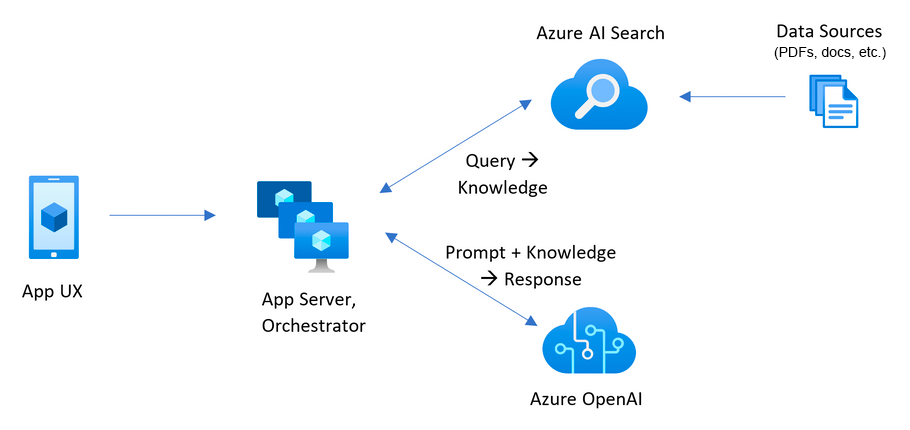
\includegraphics[width=0.6\textwidth]{figs/appcomponents.png}
    \caption{Figure to put somewhere}
    \label{fig:CLAI_Poster_Competition}
\end{figure}

The RAG chatbot was specifically designed to respond only to queries related to the course content. Questions outside the course scope received a 'cannot answer this' response to maintain the focus and academic integrity of the tool. Additionally, the chatbot provided a link to the source of its answers, enhancing transparency and trust.

\subsection*{Chatbot Evaluation and Costs}

The quality of the chatbot's responses was satisfactory, with about 85\% of interactions leading to useful answers, and only 2-4.5\% of responses being flawed. Notably, the flawed responses were quickly identified by users through follow-up questions. Despite its imperfections, the chatbot was considered a significant improvement over traditional search methods or regular chatbots used by students. The total cost of the chatbot was approximately 600€, with actual running costs around 400€ for 20,000 interactions, showcasing its cost-effectiveness.

\subsection*{Student Feedback and Future Prospects}

The chatbot was well-received based on survey responses, with students appreciating its ability to clarify complex concepts, compare texts, and summarize content. This tool proved particularly useful for large classes and when copyright for the necessary materials was held by the course instructor. Plans are in place to continue and enhance this service in future courses, focusing on guiding students to ask more effective questions.

\subsection*{Conclusion}

The implementation of the RAG chatbot at Aarhus University exemplifies the practical application of LLMs in enhancing educational experiences. The project set a precedent for future educational tools that leverage AI to support learning and inquiry. This initiative highlights the synergy between innovative technology and traditional educational practices, paving the way for more dynamic and interactive learning environments.
\chapter{Architecture of BART}
    \label{appendix:BART}
    One can inspect the model architecture by using the \texttt{transformers} library by Hugging Face.
    \section*{BART-Base}
    \begin{listing}[H]
        \begin{minted}{python}
from transformers import AutoModelForSeq2SeqLM
model_checkpoint = "facebook/bart-base"
model = AutoModelForSeq2SeqLM.from_pretrained(model_checkpoint)
        \end{minted}
        \caption{Loading pre-trained BART-base model from the Hugging Face model repository}
        \label{lst:bart_base_fetch}
    \end{listing}
    This code snippet fetches the configuration, tokenizer, and weights of the BART model from the Hugging Face model repository. The model can be inspected by printing the model object, which will output the model architecture as shown in Listing \ref{lst:bart_base_architecture}.
    \newpage
    \begin{listing}[H]
                \begin{minted}[fontsize=\footnotesize]{python}
BartForConditionalGeneration(
  (model): BartModel(
    (shared): Embedding(50265, 768, padding_idx=1)
    (encoder): BartEncoder(
      (embed_tokens): BartScaledWordEmbedding(50265, 768, padding_idx=1)
      (embed_positions): BartLearnedPositionalEmbedding(1026, 768)
      (layers): ModuleList(
        (0-5): 6 x BartEncoderLayer(
          (self_attn): BartSdpaAttention(
            (k_proj): Linear(in_features=768, out_features=768, bias=True)
            (v_proj): Linear(in_features=768, out_features=768, bias=True)
            (q_proj): Linear(in_features=768, out_features=768, bias=True)
            (out_proj): Linear(in_features=768, out_features=768, bias=True)
          )
          (self_attn_layer_norm): LayerNorm((768,), eps=1e-05, elementwise_affine=True)
          (activation_fn): GELUActivation()
          (fc1): Linear(in_features=768, out_features=3072, bias=True)
          (fc2): Linear(in_features=3072, out_features=768, bias=True)
          (final_layer_norm): LayerNorm((768,), eps=1e-05, elementwise_affine=True)
        )
      )
      (layernorm_embedding): LayerNorm((768,), eps=1e-05, elementwise_affine=True)
    )
    (decoder): BartDecoder(
      (embed_tokens): BartScaledWordEmbedding(50265, 768, padding_idx=1)
      (embed_positions): BartLearnedPositionalEmbedding(1026, 768)
      (layers): ModuleList(
        (0-5): 6 x BartDecoderLayer(
          (self_attn): BartSdpaAttention(
            (k_proj): Linear(in_features=768, out_features=768, bias=True)
            (v_proj): Linear(in_features=768, out_features=768, bias=True)
            (q_proj): Linear(in_features=768, out_features=768, bias=True)
            (out_proj): Linear(in_features=768, out_features=768, bias=True)
          )
          (activation_fn): GELUActivation()
          (self_attn_layer_norm): LayerNorm((768,), eps=1e-05, elementwise_affine=True)
          (encoder_attn): BartSdpaAttention(
            (k_proj): Linear(in_features=768, out_features=768, bias=True)
            (v_proj): Linear(in_features=768, out_features=768, bias=True)
            (q_proj): Linear(in_features=768, out_features=768, bias=True)
            (out_proj): Linear(in_features=768, out_features=768, bias=True)
          )
          (encoder_attn_layer_norm): LayerNorm((768,), eps=1e-05, elementwise_affine=True)
          (fc1): Linear(in_features=768, out_features=3072, bias=True)
          (fc2): Linear(in_features=3072, out_features=768, bias=True)
          (final_layer_norm): LayerNorm((768,), eps=1e-05, elementwise_affine=True)
        )
      )
      (layernorm_embedding): LayerNorm((768,), eps=1e-05, elementwise_affine=True)
    )
  )
  (lm_head): Linear(in_features=768, out_features=50265, bias=False)
)
                \end{minted}
                \caption{BART-base model architecture}
                \label{lst:bart_base_architecture}
            \end{listing}
The model has a total of \(139\) million parameters.

\section*{BART-Large}
Similarly, for the BART-large model:
\begin{listing}[H]
    \begin{minted}{python}
from transformers import AutoModelForSeq2SeqLM
model_checkpoint = "facebook/bart-large"
model = AutoModelForSeq2SeqLM.from_pretrained(model_checkpoint)
    \end{minted}
    \caption{Loading pre-trained BART-large model from the Hugging Face model repository}
    \label{lst:bart_large_fetch}
\end{listing}
    The model architecture is shown in Listing \ref{lst:bart_large_architecture}.
        \begin{listing}[H]
                \begin{minted}[fontsize=\footnotesize]{python}
BartForConditionalGeneration(
  (model): BartModel(
    (shared): Embedding(50265, 1024, padding_idx=1)
    (encoder): BartEncoder(
      (embed_tokens): BartScaledWordEmbedding(50265, 1024, padding_idx=1)
      (embed_positions): BartLearnedPositionalEmbedding(1026, 1024)
      (layers): ModuleList(
        (0-11): 12 x BartEncoderLayer(
          (self_attn): BartSdpaAttention(
            (k_proj): Linear(in_features=1024, out_features=1024, bias=True)
            (v_proj): Linear(in_features=1024, out_features=1024, bias=True)
            (q_proj): Linear(in_features=1024, out_features=1024, bias=True)
            (out_proj): Linear(in_features=1024, out_features=1024, bias=True)
          )
          (self_attn_layer_norm): LayerNorm((1024,), eps=1e-05, elementwise_affine=True)
          (activation_fn): GELUActivation()
          (fc1): Linear(in_features=1024, out_features=4096, bias=True)
          (fc2): Linear(in_features=4096, out_features=1024, bias=True)
          (final_layer_norm): LayerNorm((1024,), eps=1e-05, elementwise_affine=True)
        )
      )
      (layernorm_embedding): LayerNorm((1024,), eps=1e-05, elementwise_affine=True)
    )
    (decoder): BartDecoder(
      (embed_tokens): BartScaledWordEmbedding(50265, 1024, padding_idx=1)
      (embed_positions): BartLearnedPositionalEmbedding(1026, 1024)
      (layers): ModuleList(
        (0-11): 12 x BartDecoderLayer(
          (self_attn): BartSdpaAttention(
            (k_proj): Linear(in_features=1024, out_features=1024, bias=True)
            (v_proj): Linear(in_features=1024, out_features=1024, bias=True)
            (q_proj): Linear(in_features=1024, out_features=1024, bias=True)
            (out_proj): Linear(in_features=1024, out_features=1024, bias=True)
          )
          (activation_fn): GELUActivation()
          (self_attn_layer_norm): LayerNorm((1024,), eps=1e-05, elementwise_affine=True)
          (encoder_attn): BartSdpaAttention(
            (k_proj): Linear(in_features=1024, out_features=1024, bias=True)
            (v_proj): Linear(in_features=1024, out_features=1024, bias=True)
            (q_proj): Linear(in_features=1024, out_features=1024, bias=True)
            (out_proj): Linear(in_features=1024, out_features=1024, bias=True)
          )
          (encoder_attn_layer_norm): LayerNorm((1024,), eps=1e-05, elementwise_affine=True)
          (fc1): Linear(in_features=1024, out_features=4096, bias=True)
          (fc2): Linear(in_features=4096, out_features=1024, bias=True)
          (final_layer_norm): LayerNorm((1024,), eps=1e-05, elementwise_affine=True)
        )
      )
      (layernorm_embedding): LayerNorm((1024,), eps=1e-05, elementwise_affine=True)
    )
  )
  (lm_head): Linear(in_features=1024, out_features=50265, bias=False)
)
                \end{minted}
                \caption{BART-large model architecture}
                \label{lst:bart_large_architecture}
            \end{listing}
    The model has a total of \(406\) million parameters.

\end{document}
